% CVPR 2026 Paper Template; see https://github.com/cvpr-org/author-kit

\documentclass[10pt,twocolumn,letterpaper]{article}

%%%%%%%%% PAPER TYPE  - PLEASE UPDATE FOR FINAL VERSION
% \usepackage{cvpr}              % To produce the CAMERA-READY version
\usepackage[review]{cvpr}      % To produce the REVIEW version
\usepackage{tabularx}
\usepackage{enumitem}
% \usepackage[pagenumbers]{cvpr} % To force page numbers, e.g. for an arXiv version

% Import additional packages in the preamble file, before hyperref
%% This file contains a number of tweaks that are typically applied to the main document.
%% They are not enabled by default, but can be enabled by uncommenting the relevant lines.

%%
%% Inline annotations; for predefined colors, refer to "dvipsnames" in the xcolor package:
%% https://tinyurl.com/overleaf-colors
%%
\newcommand{\red}[1]{{\color{red}#1}}
\newcommand{\todo}[1]{{\color{red}#1}}
\newcommand{\TODO}[1]{\textbf{\color{red}[TODO: #1]}}
%%
%% disable for camera ready / submission by uncommenting these lines  
%%
% \renewcommand{\TODO}[1]{}
% \renewcommand{\todo}[1]{#1}

%%
%% work harder in optimizing text layout. Typically shrinks text by 1/6 of page, enable
%% it at the very end of the writing process, when you are just above the page limit
%%
% \usepackage{microtype}

%%
%% fine-tune paragraph spacing
%%
% \renewcommand{\paragraph}[1]{\vspace{.5em}\noindent\textbf{#1.}}

%%
%% globally adjusts space between figure and caption
%%
% \setlength{\abovecaptionskip}{.5em}


%%
%% Allows "the use of \paper to refer to the project name"
%% with automatic management of space at the end of the word
%%
% \usepackage{xspace}
% \newcommand{\paper}{ProjectName\xspace}

%%
%% Commonly used math definitions
%%
% \DeclareMathOperator*{\argmin}{arg\,min}
% \DeclareMathOperator*{\argmax}{arg\,max}

%%
%% Tigthen underline
%%
% \usepackage{soul}
% \setuldepth{foobar}

% It is strongly recommended to use hyperref, especially for the review version.
% hyperref with option pagebackref eases the reviewers' job.
% Please disable hyperref *only* if you encounter grave issues, 
% e.g. with the file validation for the camera-ready version.
%
% If you comment hyperref and then uncomment it, you should delete *.aux before re-running LaTeX.
% (Or just hit 'q' on the first LaTeX run, let it finish, and you should be clear).
\definecolor{cvprblue}{rgb}{0.21,0.49,0.74}
\usepackage[pagebackref,breaklinks,colorlinks,allcolors=cvprblue]{hyperref}

%%%%%%%%% PAPER ID  - PLEASE UPDATE
\def\paperID{10} % *** Enter the Paper ID here
\def\confName{CVPR}
\def\confYear{2026}

%%%%%%%%% TITLE - PLEASE UPDATE
\title{Pseudo-Hierarchies Improve Optimization Hyperparameter Robustness in Fine-Grained Image Recognition}

%%%%%%%%% AUTHORS - PLEASE UPDATE
\author{First Author\\
Institution1\\
Institution1 address\\
{\tt\small firstauthor@i1.org}
% For a paper whose authors are all at the same institution,
% omit the following lines up until the closing ``}''.
% Additional authors and addresses can be added with ``\and'',
% just like the second author.
% To save space, use either the email address or home page, not both
\and
Second Author\\
Institution2\\
First line of institution2 address\\
{\tt\small secondauthor@i2.org}
}

\begin{document}
\maketitle
\begin{abstract}
The backbone is an important component of a fine-grained image recognition system. While transformers have made significant progress in academic benchmarks, real-world deployments continue to rely on traditional CNN backbones. Our study reveals a key reason: many modern backbones exhibit pronounced sensitivity to hyperparameter settings, undermining their robustness in practical scenarios or increasing hyperparameter search costs. Hierarchical labels can mitigate this issue by regularizing the optimization process, but such annotations are rarely available—especially in specialized domains like leaf cultivar identification. Therefore, we introduce Hungarian Pseudo-Hierarchies (HPH), a training framework designed to inject hierarchical structure without requiring explicit label taxonomies. HPH begins by extracting features using a pretrained backbone, then aggregates each fine-grained class into compact clusters. A Hungarian bipartite matching module assigns these clusters to a reduced set of pseudo-classes, yielding a set of pseudo-hierarchical targets for all training samples. Finally, a fine-tuning stage leverages any standard hierarchy-aware training strategy to incorporate this synthetic structure. Across diverse settings—21 backbones, 4 fine-grained datasets, and a sweep of commonly tuned optimization hyperparameters—incorporating hierarchical biases enhances robustness to hyperparameter choices by increasing the average accuracy and reducing the standard deviation, and therefore reducing hyperparameter searches costs.
\end{abstract}

\section{Introduction}
\label{sec_introduction}

Fine-grained image recognition tasks—such as distinguishing bird species or car models—require recognizing subtle visual differences between closely related categories. In these settings, the choice of backbone architecture is a central design decision \cite{kornblith_better_2019,ye_image_2024,jeevan_which_2025}. Prior work has often attributed the strong performance of convolutional neural networks (CNNs) \cite{he_deep_2015} on datasets such as FGVC-Aircraft \cite{maji_fine-grained_2013} or Stanford Cars \cite{krause_3d_2013} to architectural properties like convolutional inductive biases that favor localized pattern recognition \cite{ye_image_2024}. This view is also reflected in practice: despite the dominance of Vision Transformers in academic benchmarks, CNNs remain widely used in real-world workflows, appearing in over 70\% of competition solutions according to an analysis of Kaggle competitions \cite{carlens_state_nodate, carlens_state_nodate-1, carlens_state_nodate-2}. However, our experiments in Section \ref{sec_results} show that Vision Transformers \cite{dosovitskiy_image_2021} can achieve competitive performance on these fine-grained datasets. ViTs' underperformance can be due to strong sensitivity to optimization hyperparameters—such as learning rate, weight decay, and optimizer choice—which can lead to suboptimal results under commonly used defaults and create the misleading impression that a model family is poorly suited to the task. Furthermore, hyperparameter searches are costly and contribute significantly to the carbon footprint of deep learning pipelines \cite{strubell_energy_2019, lacoste_quantifying_2019}, making hyperparameter robustness a necessity for efficient training of models.

To address this issue, we incorporate hierarchical training objectives aligned with the structured label spaces common in fine-grained image recognition such as biological taxonomy. Instead of relying solely on flat cross-entropy at the finest level, hierarchical losses introduce supervision across multiple semantic levels (e.g., genus, family, species). This multi-level signal provides denser and more stable gradients, effectively regularizing optimization by guiding models through a coarse-to-fine learning process. As a result, the training dynamics become less sensitive to specific hyperparameter choices, reducing variance across configurations and enabling a fairer comparison of backbone architectures.

% previous backbone benchmarks \cite{kornblith_better_2019, goldblum_battle_2023,jeevan_which_2025},

% Fine-grained image recognition (FGIR) aims to distinguish between visually similar subcategories within a broader class. Although these categories are often organized hierarchically, early FGIR methods treat labels as flat categories \cite{zhang_part-based_2014, zheng_learning_2017}, ignoring semantic structure and resulting in suboptimal performance \cite{chen_fine-grained_2018}. Hierarchical FGIR addresses this by leveraging multi-level semantic relationships, using coarse-level predictions to guide fine-grained classification \cite{chen_fine-grained_2018, chang_your_2021}. However, these methods overlook a fundamental factor: the backbone.

% This limits their ability to exploit hierarchical cues, resulting in suboptimal performance \cite{chen_fine-grained_2018}. 

% Several approaches have explored this direction, such as granularity specific classifiers \cite{chang_your_2021} and hierarchically discriminative loss functions \cite{chen_fine-grained_2018}. 

% The backbone impact has been previously studied for general image classification \cite{kornblith_better_2019, goldblum_battle_2023, jeevan_which_2025} and weakly supervised FGIR \cite{ye_image_2024}, but its role in hierarchical FGIR is underexplored. Most hierarchical FGIR methods continue to rely on a narrow set of backbones \cite{wang_multiple_2015, cerri_reduction_2016, chen_fine-grained_2018, chang_your_2021, chen_label_2022, chen_hierarchically_2024}, leaving open the question: \textbf{to what extent does the backbone influence FGIR performance in the presence of hierarchical labels?}

% Furthermore, the selection and sensitivity to hyperparameters of FGIR models has been neglected. It is often assumed that hyperparameters tuned on one dataset can generalize to similar targets \cite{ngiam_domain_2018}. However, common defaults for learning rate, weight decay, and other optimization parameters produce unreliable results after fine-tuning \cite{li_rethinking_2020}. Hyperparameter searches are computationally expensive and contribute significantly to the carbon footprint of deep learning pipelines \cite{strubell_energy_2019, lacoste_quantifying_2019}, making robustness to hyperparameter variation important for stable and dependable model deployment.

% In this work, we conduct \textbf{the first study on robust backbone selection for hierarchical FGIR}. We benchmark a wide range of convolutional and transformer-based models across multiple datasets and hyperparameters, showing that backbone choice has a large impact, from state-of-the-art performance (91\% wAP on CUB for ViT \cite{dosovitskiy_image_2021}), to poor results (80\% wAP on CUB for CLIP \cite{cherti_reproducible_2023}), as shown in Figure \ref{fig_four_plot}. 

% To measure the robustness to hyperparameter choices of a backbone, we use \textbf{Coefficient of Variation (CV)}. CV computes the ratio of standard deviation to average performance across different hyperparameters as a robustness metric; a lower CV indicates lower variance and higher mean across different hyperparameters. Through CV we observe that many backbones are sensitive to hyperparameters, specially transformer-based models. Importantly, we find that introducing hierarchical supervision consistently reduces CV across architectures and datasets (see Table \ref{tab:baseline_vs_hierarchy}). Hierarchical labels lowers sensitivity to hyperparameters and narrows the robustness gap between backbones, in some cases reducing CV by more than half compared to the baseline without hierarchical labels.

% However, this robustness gain relies on human-annotated hierarchies, which are time-consuming and expensive to construct; limiting the practical adoption of hierarchical FGIR. Since hierarchies increases hyperparameter robustness, we ask the question: \textbf{can robustness be achieved without a manually constructed hierarchy?} We propose a \textbf{pseudo-hierarchy} strategy that builds hierarchical structure systematically from feature representations and existing fine-grained labels. Our approach constructs hierarchies in a bottom-up manner by grouping fine-level classes into coarser categories using bipartite matching. Through experiments, we show that pseudo-hierarchies provide robustness improvements comparable to human-annotated hierarchies without requiring annotation costs.

Our study offers three main contributions: 
\begin{enumerate} [topsep=3pt, itemsep=2pt, parsep=1pt]
    \item We study 21 pretrained backbones (11 CNNs, 10 ViTs) across four fine-grained image recognition datasets. Our results show that many backbones are sensitive to optimization hyperparameter choices. 
    % This may impact perception of a model family's performance for a given task, despite the fact %The right choice of backbone can \textbf{change accuracy by up to 13\%}.
    \item We evaluate hierarchical supervision across backbones and datasets. Hierarchy consistently improves optimization hyperparameter robustness, as measured by the coefficient of variations (CV) of the accuracy, by reducing CV up to \textbf{75\%} compared to FGIR baselines.
    \item We propose Hungarian Pseudo-Hierarchy (HPH), a novel pseudo-hierarchy construction strategy that alleviates the cost of manual annotation and enables incorporating hierarchical inductive biases into datasets without an explicit hierarchy. Experiments show that pseudo-hierarchies can improve robustness, reducing CV by up to \textbf{50\%}.
\end{enumerate}



\section{Related Works}
\label{sec_related}
\subsection{Fine-Grained Image Recognition (FGIR)}
Early FGIR methods relied on part annotations or bounding boxes to guide localization \cite{zhang_part-based_2014}. While effective, these methods are difficult to scale due to the cost of annotations. Later works leveraged image-level labels with attention mechanisms, such as MA-CNN \cite{zheng_learning_2017}, which learned part-aware features without extra supervision. However, these methods often employ multi-stage pipelines involving zooming-in and cropping discriminative areas, which significantly increases the cost.
% However, these models ignored class hierarchies, limiting their ability to capture semantic structure and generalize across categories.

Kornblith et al. \cite{kornblith_better_2019} and follow-up work \cite{goldblum_battle_2023, jeevan_which_2025} demonstrated that the backbone can make as much of a difference as a specialized discriminative part selection method. Ye et al. \cite{ye_image_2024} investigated backbones for weakly supervised FGIR and concluded that CNN backbones are more suitable for machine-like tasks such as aircraft and cars classification. But our results on Section \ref{sec_results} show that ViTs can be competitive to CNNs even in this tasks; the reason why ViTs may be perceived inferior in these tasks is due to sensitivity to optimization hyperparameters.

% \subsection{Backbone effect on FGIR}
% Kornblith et al. \cite{kornblith_better_2019} analyzed whether higher ImageNet accuracy leads to better downstream performance. Th while Goldblum et al. \cite{goldblum_battle_2023} and Jeevan et al. \cite{jeevan_which_2025} focused on the impact of backbone in general image classification. Ye et al. \cite{ye_image_2024} investigated backbones for weakly supervised FGIR and concluded that CNN backbones are more suitable for machine-like tasks such as aircraft and cars classification. But our results on Section 

% Recent works have explored the impact of backbone architectures on transfer learning and FGIR. Kornblith et al. \cite{kornblith_better_2019} analyzed whether higher ImageNet accuracy leads to better downstream performance, while Goldblum et al. \cite{goldblum_battle_2023} and Jeevan et al. \cite{jeevan_which_2025} focused on the impact of backbone in general image classification. Ye et al. \cite{ye_image_2024} investigated backbones for weakly supervised FGIR. However, these works neglect the impact of hierarchical labels and robustness to hyperparameter choices for the backbones. Our work systematically investigates how backbone choice interacts with hierarchy and to evaluate robustness across hyperparameters, offering new insights for hierarchical FGIR.

\subsection{Hierarchical Fine-Grained Image Recognition}
Hierarchical FGIR methods can address hyperparameter sensitivity by introducing inductive biases that act as regularization in the form of multi-level prediction heads and hierarchy-aware losses. One of the first works, Multi-Granularity Descriptor (MGD) \cite{wang_multiple_2015}, used weakly supervised taxonomic descriptors. This was followed by methods such as, Hierarchical Semantic Embedding (HSE) \cite{chen_fine-grained_2018} and granularity-specific classifiers \cite{chang_your_2021}, which introduced hierarchy-aware loss functions and multi-level prediction heads. Although effective, these methods still struggle with class ambiguity within coarse groups and rely on a narrow set of backbone architectures.

\subsection{Hierarchically Consistent Learning}
Hierarchically consistent learning enforces compatibility between predictions at different hierarchy levels through architectures or loss functions. Early work such as Hierarchical Semantic Embedding (HSE) by Chen et al. \cite{chen_fine-grained_2018} sequentially predicts category levels and uses higher-level predictions as soft constraints to regularize lower-level output. Hierarchical Residual Network (HRN) \cite{chen_label_2022} proposed injecting coarse-level features into finer-level through residual connections, allowing parent-category information to guide fine-grained recognition. 

Later approaches extend consistency enforcement through different mechanisms, such as Semantics-Aware Hierarchical Consensus (SAHC) \cite{weikmann_semantics-aware_2025} aligns predictions from multiple hierarchy levels through a consensus distribution optimized via divergence minimization, improving robustness under bad hierarchies. Free-Grained Hierarchical Recognition \cite{park_free-grained_2025} addresses mixed-granularity supervision using vision–language models to propagate semantic information across hierarchy levels. 
% Beyond single-label, Hierarchy-Consistent Adaptive Loss (HCAL) \cite{hcal} aggregates child representations into parent prototypes and adaptively balances multi-level objectives to reduce hierarchy mismatches.

Collectively, these works demonstrate that explicitly enforcing hierarchical agreement can increase performance and robustness. Our method is complementary to these approaches; our method creates pseudo-hierarchies which can be integrated with existing hierarchical training frameworks, enabling incorporating hierarchical inductive biases into datasets without predefined hierarchies.

\subsection{Pseudo-Hierarchies in Image Classification}
Pseudo-hierarchies are widely used across different image classification tasks, from unsupervised person re-identification (re-ID) to HFGIR. These methods construct hierarchical structures from data representations to improve learning efficiency. In unsupervised re-ID, Online Hierarchical Cluster Dynamics \cite{zheng_online_2021} forms a bottom-up hierarchy from feature embeddings that evolves during training. Logits-to-Hierarchy (L2H) \cite{palumbo_logits_2025} derives hierarchical class structures by clustering classifier logits to recover semantic taxonomies without retraining. Deep Taxonomic Networks \cite{wang_deep_2025} learn hierarchical organization by imposing a tree-structured Gaussian mixture prior over latent representations, while pseudo-fine labels can also be constructed under coarse supervision using feature clustering \cite{hsieh_pseudo-label_2019}.

Existing methods follow a coarse-to-fine (top-down) clustering approach, whereas our method constructs pseudo-hierarchies from feature representations of pretrained models and existing fine labels, merging categories into coarser groups (bottom-up) to facilitate optimization of backbones under fine-grained conditions.
% to leverage pseudo-hierarchies specifically adapted for fine-grained recognition.



\section{Learning with Hungarian Pseudo-Hierarchies}
\label{sec_method}
Our approach consists of three stages. First, feature representations are extracted from pretrained backbones. Second, Hungarian Pseudo-Hierarchies (HPH) are constructed by clustering fine-grained classes into coarse classes based on their feature representations. Finally, the resulting hierarchy is used within a hierarchical module for training and prediction. The following subsections describe feature extraction, pseudo-hierarchy construction, and hierarchical module.

\subsection{Feature Representation Extraction}
Features are extracted from pretrained backbones. For CNN-based models (ResNet50 variants), features are extracted from the last BatchNorm layer of the final residual block, while for Transformer-based models (ViT-B variants) features are obtained from the last LayerNorm of the encoder. Feature vectors are pooled with adaptive average pooling to ensure a consistent output shape.

Let \(x\) be an input image and \(\phi(\cdot)\) the feature extractor. The extracted representation for a single image is
\[
\mathbf{z} = \phi(x) \in \mathbb{R}^{C},
\]
where \(C\) is the number of feature channels. Collecting features across all images in a dataset yields a feature matrix
\[
Z \in \mathbb{R}^{S \times C},
\]
where \(S\) is the number of samples. These features preserve semantic information at the fine-grained class level and provide a foundation for clustering-based hierarchy construction.


\subsection{Pseudo-Hierarchy Construction}
To alleviate the cost of manually annotating hierarchical labels, we propose \textbf{Hungarian Pseudo-Hierarchies (HPH)}, a method that constructs pseudo-hierarchies from fine-grained labels by formulating coarse-level grouping as a bipartite matching problem. The resulting coarse labels are mapped to fine classes, producing a hierarchy that can be integrated with any hierarchical FGIR module.

Given feature representations extracted from a pretrained backbone, each fine class \(f_i\) is represented by its centroid:
\[
\mathbf{c}_i = \frac{1}{|k_i|} \sum_{x \in k_i} \phi(x),
\]
where \(k_i\) denotes the set of samples belonging to fine class \(i\), and \(\phi(x) \in \mathbb{R}^{d}\) is the \(d\)-dimensional feature embedding (channel representation) extracted from sample \(x\). Each centroid \(\mathbf{c}_i\) lies in the same feature space as the backbone feature representations.

We then compute the pairwise Euclidean distance between centroids to form a cost matrix:
\[
C_{ij} = \sqrt{\sum_{m=1}^{d} (c_{i,m} - c_{j,m})^2}, \quad C \in \mathbb{R}^{N \times N},
\]
where \(N\) is the number of fine classes.

Since the desired number of coarse classes \(L\) is smaller than \(N\), we pad the cost matrix with the maximum distance for the extra columns. The Hungarian algorithm \cite{kuhn_hungarian_1955} is then applied to find the optimal one-to-one assignments between fine and coarse classes. Fine classes assigned to padded columns are reassigned to the nearest valid coarse cluster based on centroid distance. This procedure generates a 2-level pseudo-hierarchy for a dataset.

\subsection{Hierarchical Classification Module}
Given a hierarchy constructed either from manual annotation or the proposed pseudo-hierarchy generation process, prediction is performed using a hierarchical multi-granularity classification framework following Chang et al. \cite{chang_your_2021}. In this setting, each image is associated with labels ordered from coarse to fine granularity. The objective is a multi-task learning problem in which classifiers at different semantic levels are learned jointly.

Separate classification heads are assigned to each hierarchy level, enabling independent prediction of coarse- and fine-level labels. This design disentangles the decision spaces across different hierarchical levels, allowing each classifier to specialize in recognizing patterns relevant to its semantic level.

Let the backbone network produce a feature representation $\mathbf{z}$ for an input image $x$. For a hierarchy with $K$ levels, the shared feature is forwarded to $K$ classification heads ${g_k(\cdot)}_{k=1}^{K}$, where each head predicts a probability distribution over the label space of its corresponding level with the formula below:
\[
\mathbf{p}^{(k)} = g_k(\mathbf{z}), \quad k = 1, \dots, K,
\]

Training is performed using $\mathcal{L}_{\text{CE}}$ computed independently at every hierarchy level. The overall hierarchical loss is the sum of per-level losses:
\[
\mathcal{L} = \sum_{k=1}^{K} \mathcal{L}_{\mathrm{CE}}^{(k)}
\]
Each classifier therefore contributes to the overall optimization while sharing the same backbone representation.

The aggregated loss supervises predictions across all levels in the hierarchy, encouraging the learned representation to remain consistent with the hierarchical structure. During inference, the model outputs one prediction per level. The collection of predictions across levels forms the final hierarchical output, completing the classification process.

\section{Experiment Setup}
\label{sec_methodology}
We evaluate our approach on four datasets: \textbf{FGVC Aircraft} \cite{maji_fine-grained_2013}, \textbf{CUB-200-2011}, \textbf{Soylocal} \cite{wah_caltech-ucsd_2011}, and \textbf{Stanford Cars} \cite{krause_collecting_nodate}. Real hierarchies are constructed from Wikipedia class taxonomies following Chang et al. \cite{chang_your_2021}.

Our experiments consider 21 backbones spanning two types, 10 Transformer (ViT-B) and 11 CNN (ResNet50), covering a broad range of training methods, including fully supervised (FSL), semi-supervised (SemiSL), and self-supervised learning (SSL).  
Here are the exact models used:
\begin{itemize} [topsep=3pt, itemsep=2pt, parsep=1pt]
    \item \textbf{ViT-B models}:
    \begin{itemize}[topsep=3pt, itemsep=2pt, parsep=1pt]
        \item \textbf{FSL}: ViT\cite{dosovitskiy_image_2021}, DeiT\cite{touvron_deit_2022}, DeiT3 (IN1K, IN21K)\cite{touvron_deit_2022}, MIIL \cite{ridnik_imagenet-21k_2021}
        \item \textbf{SSL (Discriminative)}: MoCoV3\cite{chen_empirical_2021}, DINO\cite{caron_emerging_2021}, CLIP-LAION5B\cite{cherti_reproducible_2023}, SigLIP-v2\cite{tschannen_siglip_2025}
        \item \textbf{SSL (Generative)}: MAE\cite{he_masked_2021}
    \end{itemize}
    \item \textbf{ResNet50 models}:
    \begin{itemize}[topsep=3pt, itemsep=2pt, parsep=1pt]
        \item \textbf{FSL}: Torchv1\cite{he_deep_2015}, Torchv2\cite{he_deep_2015}, Gluon\cite{he_bag_2018}, A1\cite{wightman_resnet_2021}, MIIL\cite{ridnik_imagenet-21k_2021}
        \item \textbf{SemiSL}: IG1B\cite{yalniz_billion-scale_2019}, YFCC100M\cite{yalniz_billion-scale_2019}
        \item \textbf{SSL (Discriminative)}: MoCoV3\cite{chen_empirical_2021}, SupCon\cite{khosla_supervised_2021}, SwAV\cite{caron_unsupervised_2021}
        \item \textbf{SSL (Generative)}: SparK\cite{tian_designing_2023}
    \end{itemize}
\end{itemize}

\begin{figure*}[!htb]
    \centering
    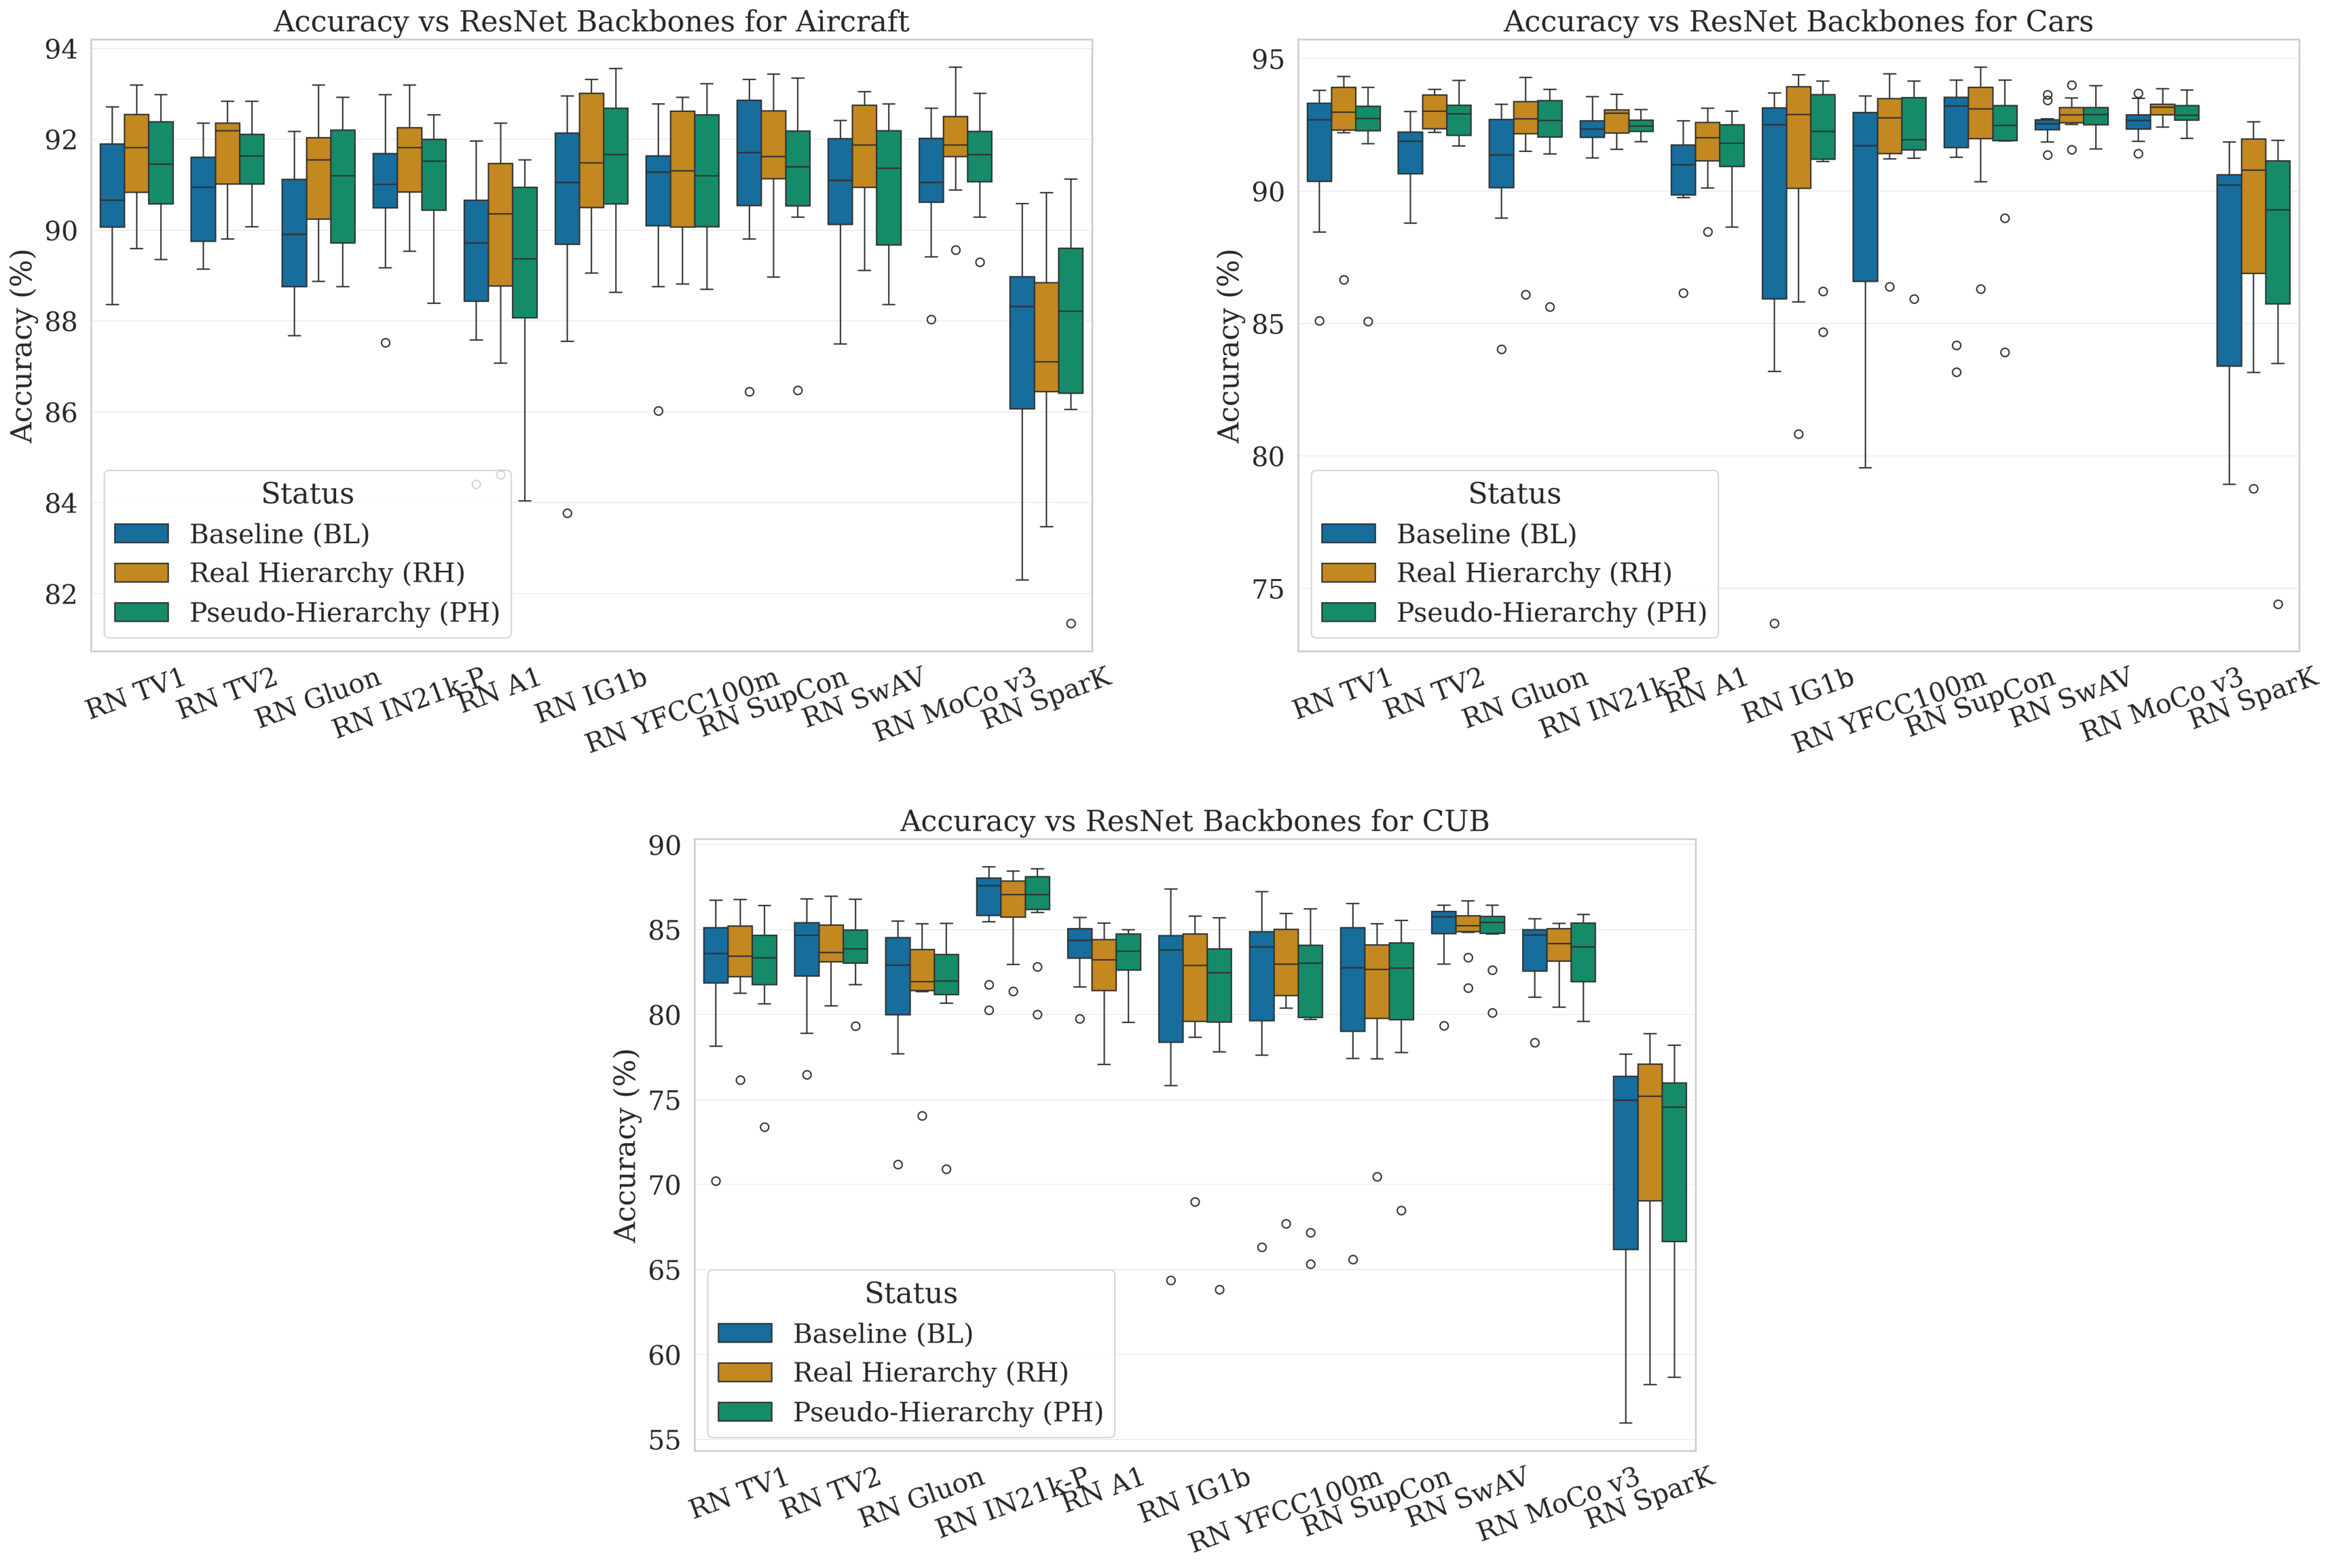
\includegraphics[width=0.95\textwidth]{figures/combined_main_plots_rn.png}
    \caption{Performance of different ResNet models across 3 settings: \textbf{Baselines} (Without hierarchy), \textbf{Real Hierarchies} and \textbf{Pseudo-Hierarchy} and 3 datasets. Pseudo-hierarchy for Aircraft and Cars use 50\% cluster ratio, while CUB uses 70\%.} 
    \label{fig_pseudo_main_rn}
\end{figure*}

\begin{figure*}[!htb]
    \centering
    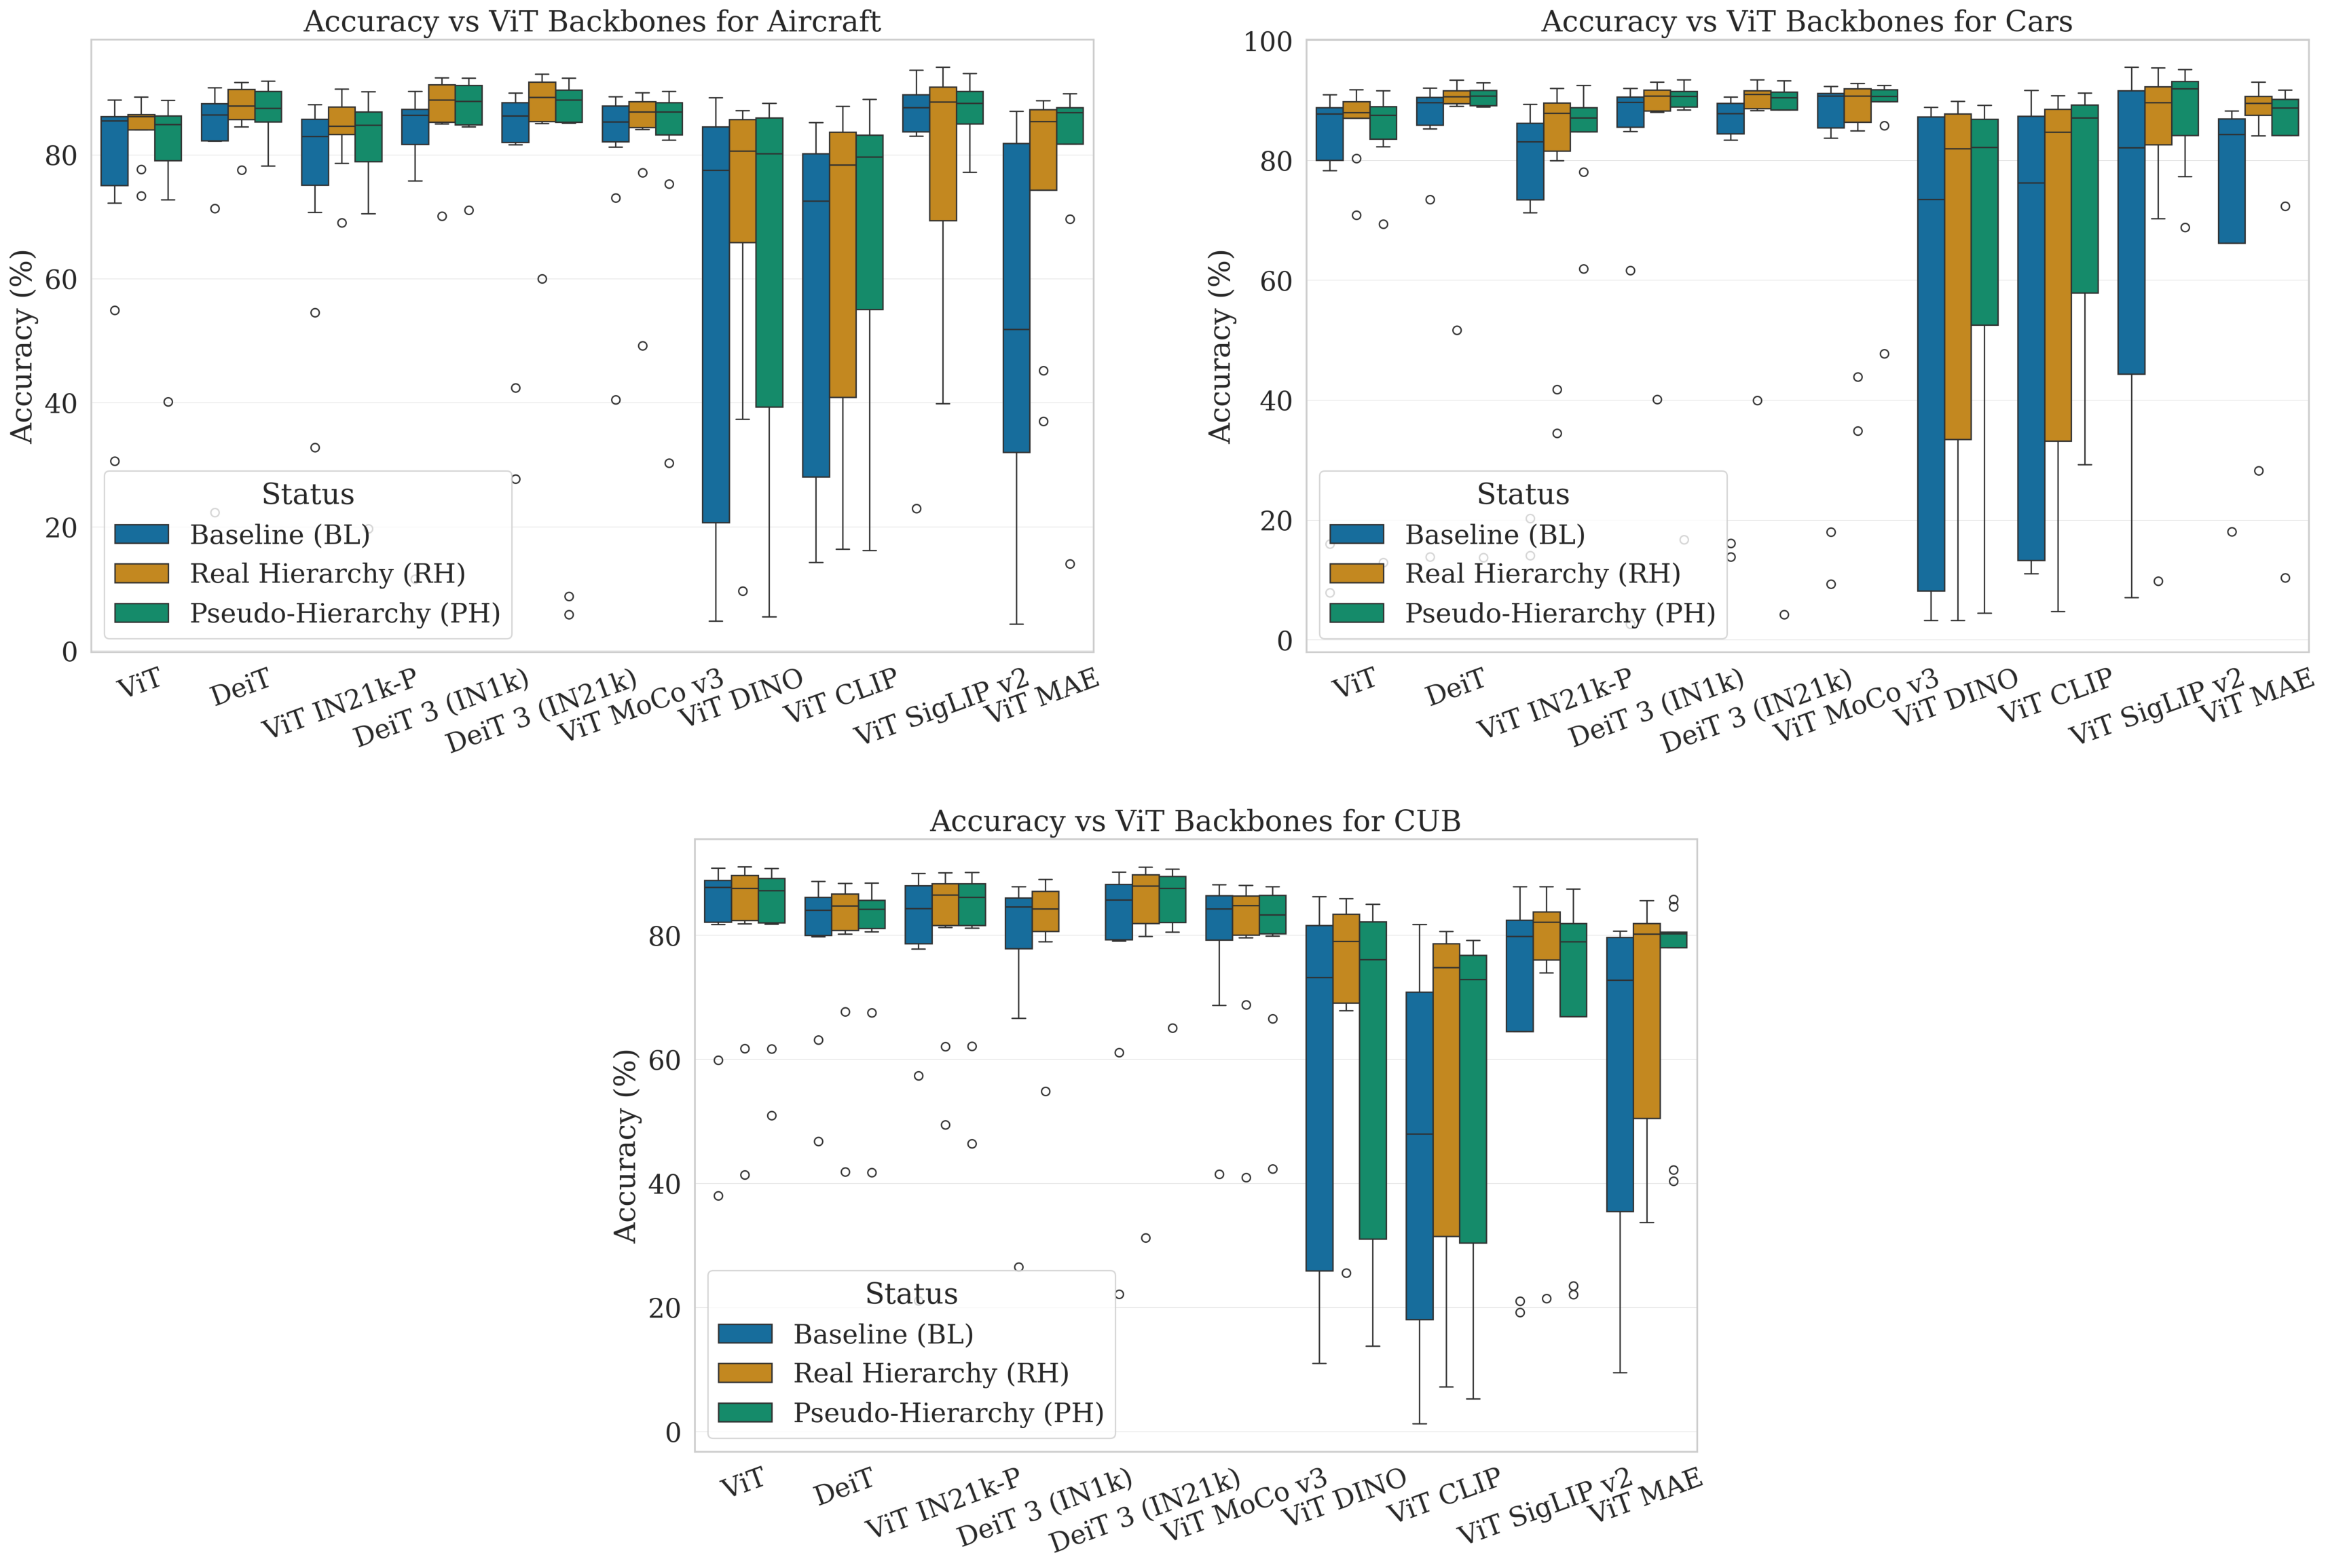
\includegraphics[width=0.95\textwidth]{figures/combined_main_plots_vit.png}
    \caption{Performance of different ViT models across 3 settings: \textbf{Baselines} (Without hierarchy), \textbf{Real Hierarchies} and \textbf{Pseudo-Hierarchy} and 3 datasets. Pseudo-hierarchy for Aircraft and Cars use 50\% cluster ratio, while CUB uses 70\%.} 
    \label{fig_pseudo_main_vit}
\end{figure*}


To assess model effectiveness in hierarchical FGIR, we measure several evaluation metrics measuring individual level accuracy and robustness:
\begin{itemize}
    % \item \textbf{Per-level accuracy}. The Top-1 classification accuracy of each level in the hierarchy. There are \textbf{3 hierarchical levels} at most, these are denoted by \textbf{L3, L2, L1, from coarsest to finest}.

    \item \textbf{Finest-level accuracy}. We report the Top-1 classification accuracy at the finest level of the hierarchy (L1). While the hierarchical structure contains up to three levels (L3, L2, and L1, from coarsest to finest), the coarse labels in the pseudo-hierarchy are automatically generated and do not correspond to ground-truth semantic labels. Therefore, coarse-level accuracies are not meaningful for evaluation. As a result, we focus our analysis on the finest-level accuracy, which reflects the true classification performance on the original dataset labels.

    % \item \textbf{Weighted Average Precision (wAP).}  
    % to address class imbalance, wAP weights per-class accuracy by sample count
    % wAP is defined as:
    % \[
    % wAP = \frac{1}{N} \sum_{k=1}^{K} n_k \cdot \text{Acc}_k
    % \]
    % where $K$ is the number of classes, $n_k$ is the number of samples in class $k$, $\text{Acc}_k$ is the accuracy for class $k$, and $N = \sum_{k=1}^{K} n_k$ is the total number of samples.
    
    \item \textbf{Coefficient of Variation (CV)}. 
    Coefficient of Variation \cite{brown_applied_1998} balances accuracy and robustness by measuring the ratio of standard deviation to mean accuracy across multiple runs.
    Coefficient of Variation is defined as:
    \[
    CV = \frac{\sigma}{\mu} \times 100\% 
    \]
    where $\mu$ denotes the mean accuracy and $\sigma$ the standard deviation across evaluation runs. Lower Coefficient of Variation indicates a model achieves both high mean accuracy and low deviation, desirable characteristics in practical deployments. 
\end{itemize}

We fine-tune our models for 200 epochs with a batch size of 8. To study the impact of hyperparameters, we use two optimizers (SGD and AdamW) across 10 learning rates, SGD (0.3–0.003) with weight decay 0, and AdamW (0.005–0.000005) with weight decay 0.05. We employ cosine learning rate scheduler and mixed precision. During training, we employ standard data augmentation (resize to 550×550, random crop to 448×448, horizontal flip). Center cropping is used during inference.

We control the granularity of coarse-level pseudo-hierarchies using a \textbf{cluster ratio}, defined as the number of coarse labels relative to the number of fine-grained labels. We construct 2-level pseudo-hierarchies with three cluster ratios: 25\%, 50\%, and 70\%. These hierarchies are used to evaluate how the number of coarse-level labels affects hierarchical FGIR performance.

\section{Results}
\label{sec_results}

% \begin{table}[!htb]
%     \centering
%     % \small
%     \caption{CV of different hyperparameters and datasets. Lower is better. Best and second best are \textbf{bold faced} and \underline{underlined}, respectively.}
%     \label{tab:ada_ratio}
%     \begin{tabularx}{\linewidth}{p{2.9cm}p{1.75cm}XX}
%         \toprule
%         Method & Fine-tuned & Frozen & Average \\
%         \midrule
%         \multicolumn{4}{>{\raggedright\arraybackslash}p{\linewidth}}{\textbf{ResNet50 models (CNN-based)}} \\
%         \multicolumn{4}{>{\raggedright\arraybackslash}p{\linewidth}}{\textit{Fully-Supervised models}} \\
%         RN TV1\cite{he_deep_2015} & 2.44 & 2.98 & 2.71 \\
%         RN TV2\cite{he_deep_2015} & 1.39 & 1.24 & 1.31 \\
%         RN Gluon\cite{he_bag_2018} & 2.61 & 1.41 & 2.01 \\
%         RN IN21k-P\cite{ridnik_imagenet-21k_2021} & 1.54 & 1.04 & \underline{1.29} \\
%         RN A1\cite{wightman_resnet_2021} & 2.42 & 0.96 & 1.69 \\
%         \multicolumn{4}{>{\raggedright\arraybackslash}p{\linewidth}}{\textit{Semi-Supervised models}} \\
%         RN IG1b\cite{yalniz_billion-scale_2019} & 4.28 & 1.18 & 2.73 \\
%         RN YFCC100m\cite{yalniz_billion-scale_2019} & 3.53 & 1.5 & 2.51 \\
%         \multicolumn{4}{>{\raggedright\arraybackslash}p{\linewidth}}{\textit{Self-Supervised models (Discriminative)}} \\
%         RN SupCon\cite{khosla_supervised_2021} & 3.24 & 1.37 & 2.31 \\
%         RN SwAV\cite{caron_unsupervised_2021} & \underline{1.33} & 1.46 & 1.39 \\
%         RN MoCo v3\cite{chen_empirical_2021} & \textbf{1.18} & 1.32 & \textbf{1.25} \\
%         \multicolumn{4}{>{\raggedright\arraybackslash}p{\linewidth}}{\textit{Self-Supervised models (Generative)}} \\
%         RN SparK\cite{tian_designing_2023} & 5.67 & 3.92 & 4.8 \\
%         \midrule
%         \multicolumn{4}{>{\raggedright\arraybackslash}p{\linewidth}}{\textbf{ViT-B models (Transformer-based)}} \\
%         \multicolumn{4}{>{\raggedright\arraybackslash}p{\linewidth}}{\textit{Fully-Supervised models}} \\
%         ViT\cite{dosovitskiy_image_2021} & 11.35 & 1.01 & 6.18 \\
%         DeiT\cite{touvron_training_2021} & 12.79 & 0.77 & 6.78 \\
%         ViT IN21k-P\cite{ridnik_imagenet-21k_2021} & 17.43 & 1.98 & 9.7 \\
%         DeiT 3 (IN1k)\cite{touvron_deit_2022} & 13.55 & 1.06 & 7.31 \\
%         DeiT 3 (IN21k)\cite{touvron_deit_2022} & 18.42 & \textbf{0.59} & 9.51 \\
%         \multicolumn{4}{>{\raggedright\arraybackslash}p{\linewidth}}{\textit{Self-Supervised models (Discriminative)}} \\
%         ViT MoCo v3\cite{chen_empirical_2021} & 20.13 & 1.24 & 10.68 \\
%         ViT DINO\cite{caron_emerging_2021} & 42.36 & 0.96 & 21.66 \\
%         ViT CLIP\cite{cherti_reproducible_2023} & 52.52 & \underline{0.63} & 26.58 \\
%         ViT SigLIP v2\cite{tschannen_siglip_2025} & 31.34 & 2.1 & 16.72 \\
%         \multicolumn{4}{>{\raggedright\arraybackslash}p{\linewidth}}{\textit{Self-Supervised models (Generative)}} \\
%         ViT MAE\cite{he_masked_2021} & 28.2 & 4.44 & 16.32 \\
%         \bottomrule
%     \end{tabularx}
% \end{table}

\subsection{Impact of Backbone, Pretraining and Hyperparameter on FGIR}
\subsubsection{Backbone Choice Drives Performance}
Fig. \ref{fig_pseudo_main_rn} and  Fig. \ref{fig_pseudo_main_vit} highlight how backbone selection alone can lead to vastly different outcomes. Among ResNets, MoCoV3 performs best (94\% wAP on Aircraft), while the worst performing one, Spark obtains 92\% wAP. ViT models show larger performance variance: SigLIP-v2 excels on Aircraft (94\%) and Cars (95\%), while original ViT excels CUB (91\%). In contrast, DINO performs worst with 87\% on Aircraft and 89\% on Cars. These findings show that backbone selection, especially for ViTs, can lead to \textbf{state-of-the-art performance or degraded results}.

\begin{figure}[ht]
    \centering
    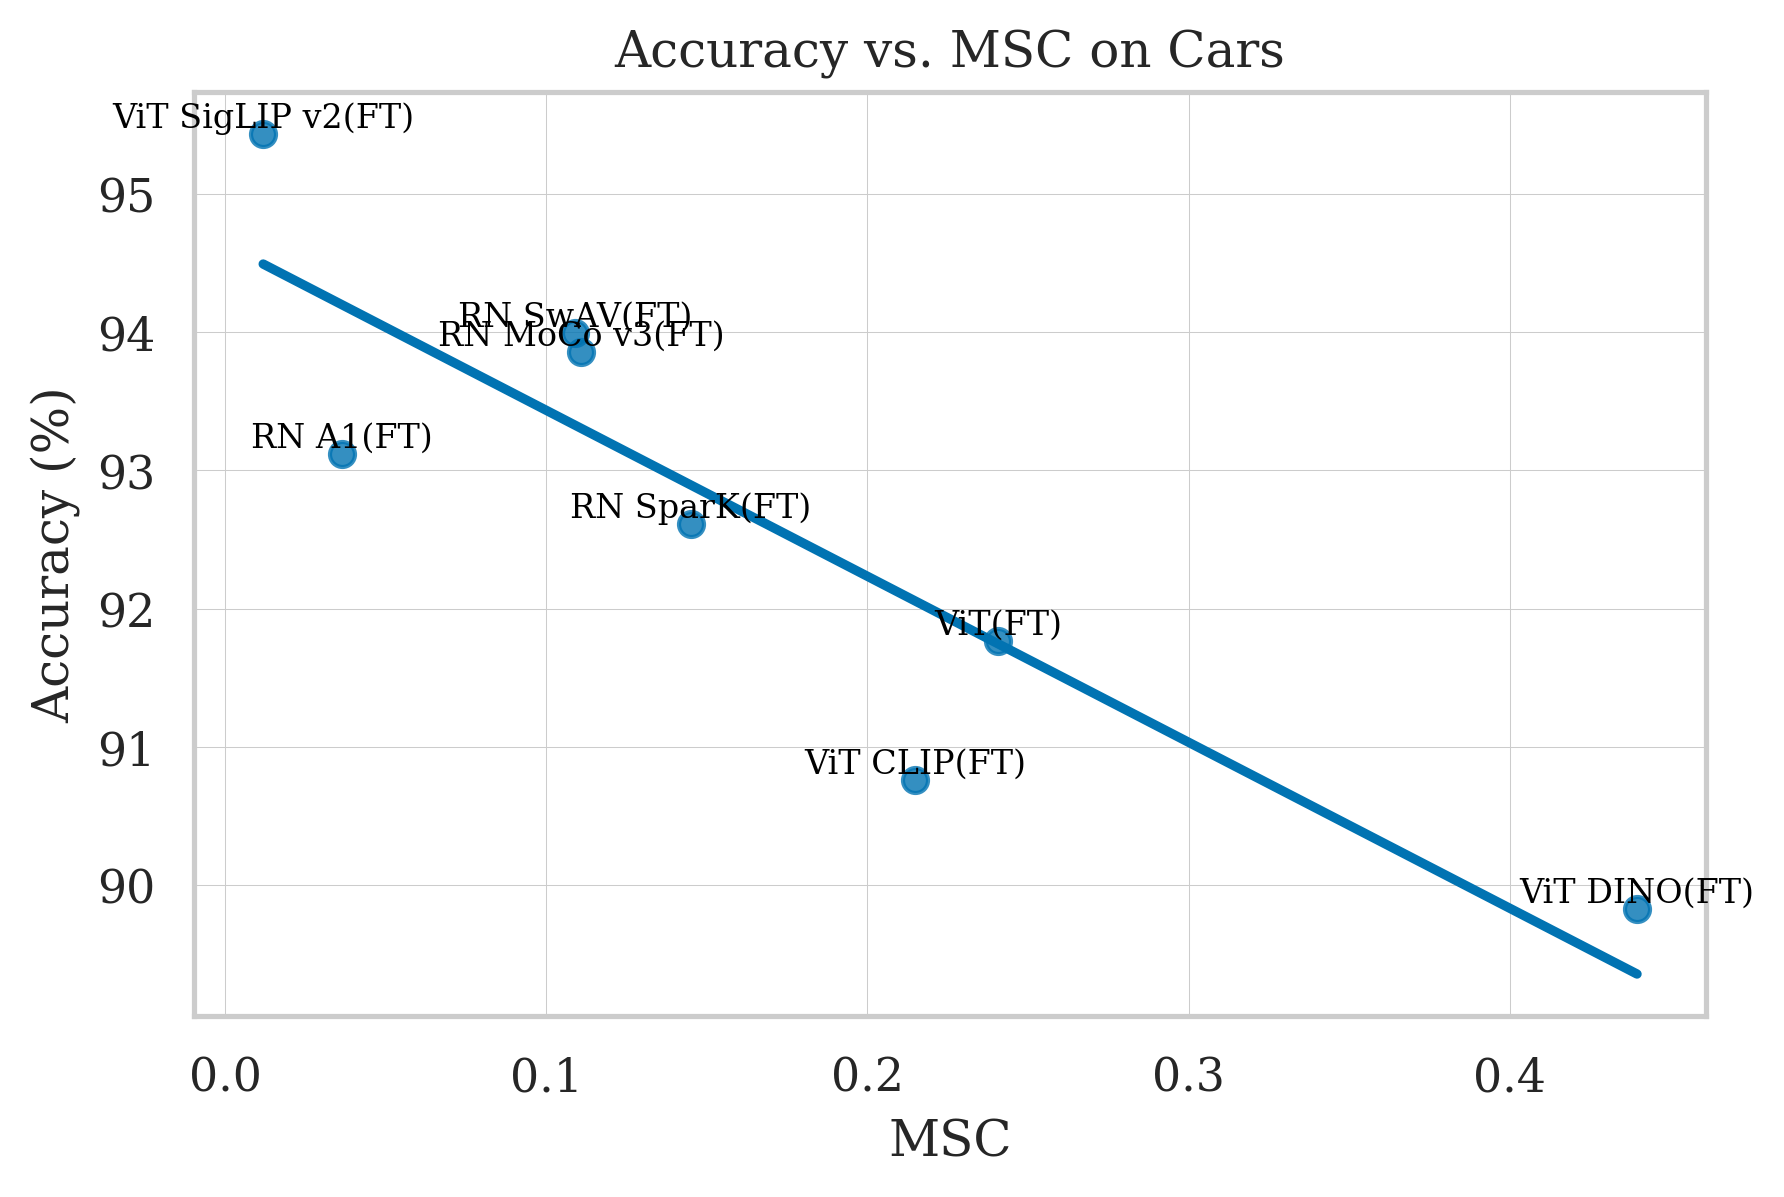
\includegraphics[width=0.875\linewidth]{figures/example_plot.png}
    \caption{Plot showing Accuracy vs. MSC for the Top-2 and Worst-2 ResNet and ViT fine-tuned models. ViT SigLiP is far away from the rest of the ViT.} 
    \label{fig_example_metric}
\end{figure}

\subsubsection{ResNet models do better on machines, but ViT models
do better on animals}
\label{sec:dataset_differences}
In Fig. \ref{fig_pseudo_main_rn} and  Fig. \ref{fig_pseudo_main_vit} \textbf{ResNet models} generally \textbf{perform better} on \textbf{Aircraft and Cars}, while \textbf{ViTs do better} on \textbf{CUB}. This aligns with Ye et al.\cite{ye_image_2024}, which suggests that \textbf{objects with more dynamic shapes} (e.g. animals) \textbf{benefit} more from the \textbf{self-attention mechanism} in transformers. In contrast, \textbf{objects with more static shapes} (e.g. machines) \textbf{benefit} from the \textbf{inductive biases} in CNNs. Also, ImageNet contains a substantial number of bird-related images, which may have contributed to a performance boost for ViT models on the CUB dataset.

However, we observe \textbf{an exception}: \textbf{SigLIPv2}, a ViT model, achieves \textbf{better performance} on \textbf{Aircraft and Cars} than the \textbf{best ResNet model}, challenging this observation. To explain this, we employ \textbf{Mean Silhouette Coefficient (MSC)} \cite{rousseeuw_silhouettes_1987}, which quantifies the quality of feature clustering based on inter-class separation\cite{islam_broad_2021} and intra-class variance\cite{islam_broad_2021}. Higher values indicate well-separated and compact class clusters, while lower values imply more ambiguous features. We plot the Top-2 and Worst-2 wAP vs MSC for clarity, as observed in \ref{fig_example_metric}, SigLIP obtains lower MSC compared to other ViTs, suggesting tighter and less distinct feature representations. We also observed that ResNets obtains lower MSC than ViTs, while SigLiP obtains lower values than ResNets. This indicates that \textbf{performance stems from learned representations during pretraining rather than only architectural biases}.

% \begin{table}[t]
% \centering
% \caption{CV ratio across hyperparameters comparing baseline without hierarchical labels vs model with hierarchical labels. Lower is better.}
% \label{tab:baseline_vs_hierarchy}
% \begin{tabularx}{\linewidth}{p{1.8615cm}XXXXXX}
% \toprule
% % \multirow{2}{*}{Method} & \multicolumn{2}{c}{Aircraft} & \multicolumn{2}{c}{Cars} & \multicolumn{2}{c}{CUB} \\
% Method & \multicolumn{2}{c}{Aircraft} & \multicolumn{2}{c}{Cars} & \multicolumn{2}{c}{CUB} \\
% \cmidrule(lr){2-3} \cmidrule(lr){4-5} \cmidrule(lr){6-7}
% Hier. Labels & - & \checkmark & - & \checkmark & - & \checkmark \\
% \midrule
% RN YFCC100m & 2.16 & 1.59 & 5.64 & 2.51 & 7.60 & 6.51 \\
% RN IG1b     & 3.08 & 1.73 & 7.51 & 0.70 & 8.67 & 6.19 \\
% RN Gluon    & 1.68 & 1.47 & 3.03 & 2.51 & 5.46 & 3.85 \\
% RN TV1      & 1.47 & 1.30 & 3.12 & 2.39 & 5.95 & 3.63 \\
% RN TV2      & 1.31 & 1.12 & 1.47 & 0.71 & 4.07 & 2.33 \\
% \midrule
% ViT              & 25.00 & 6.25 & 44.30 & 7.62 & 21.63 & 20.19 \\
% DeiT             & 26.14 & 4.29 & 29.88 & 15.24 & 17.03 & 18.21 \\
% ViT IN21k-P      & 22.73 & 7.94 & 40.56 & 27.39 & 28.29 & 16.95 \\
% DeiT 3 (IN1k)    & 30.38 & 6.75 & 35.88 & 19.93 & 24.46 & 12.93 \\
% DeiT 3 (IN21k)   & 29.01 & 11.82 & 48.65 & 20.03 & 27.38 & 23.43 \\
% ViT MAE          & 47.99 & 26.31 & 61.25 & 26.66 & 49.52 & 31.63 \\
% ViT CLIP         & 51.09 & 42.55 & 64.26 & 54.80 & 73.75 & 60.22 \\
% \bottomrule

% \end{tabularx}
% \end{table}

% \subsection{Impact of Hyperparameters}
\subsubsection{ResNet models are more robust than ViT models}
In Fig. \ref{fig_pseudo_main_rn} and  Fig. \ref{fig_pseudo_main_vit}, under \textbf{fine-tuned settings}, \textbf{ResNet models} pretrained with \textbf{discriminative objectives} (e.g., MoCoV3, SwAV) achieve the highest mean accuracy and lowest deviation. For \textbf{ViT models}, \textbf{fully supervised models} such as original ViT, DeiT, and DeiT3 also show strong fine-tuned performance with low deviation. In general, \textbf{ResNet models are more robust} than ViTs across pretraining and hyperparameter, as supported by consistently lower CVs in both figures. Among them, MoCoV3, a discriminative model, achieves the best CV across different settings. These results show discriminative ResNet models as a strong baseline for future hierarchical FGIR research.

% \subsubsection{Scale of pretraining affects frozen performance}
% In Fig. \ref{fig_pseudo_main_rn} and  Fig. \ref{fig_pseudo_main_vit}, under \textbf{frozen settings}, \textbf{Semi-Supervised models} (IG1b, YFCC300m) and the \textbf{IN21K-P model achieve the best results}.These 3 models are \textbf{pretrained on larger datasets, IG1b, YFCC300m, In21k accordingly}. For \textbf{ViT models}, \textbf{original ViT, DeiT (IN21K) and CLIP} models achieve high accuracy. They are also \textbf{pretrained} on \textbf{larger datasets}, \textbf{In21k, LAION5b accordingly}.

% \subsubsection{Generative models underperform in frozen settings}
% \textbf{Generative models} (e.g SparK, MAE) consistently \textbf{underperform in frozen settings} for both ResNet and ViT backbones, as observed in Fig. \ref{fig_pseudo_main_rn} and  Fig. \ref{fig_pseudo_main_vit}. Generative models, trained via masking and reconstruction objectives, appear to struggle with distinguishing fine-grained categories, indicating that \textbf{this strategy is not suited for frozen settings in hierarchical FGIR tasks}.

% \begin{figure*}[!htb]
%     \centering
%     \begin{minipage}{0.43\linewidth}
%         \centering
%         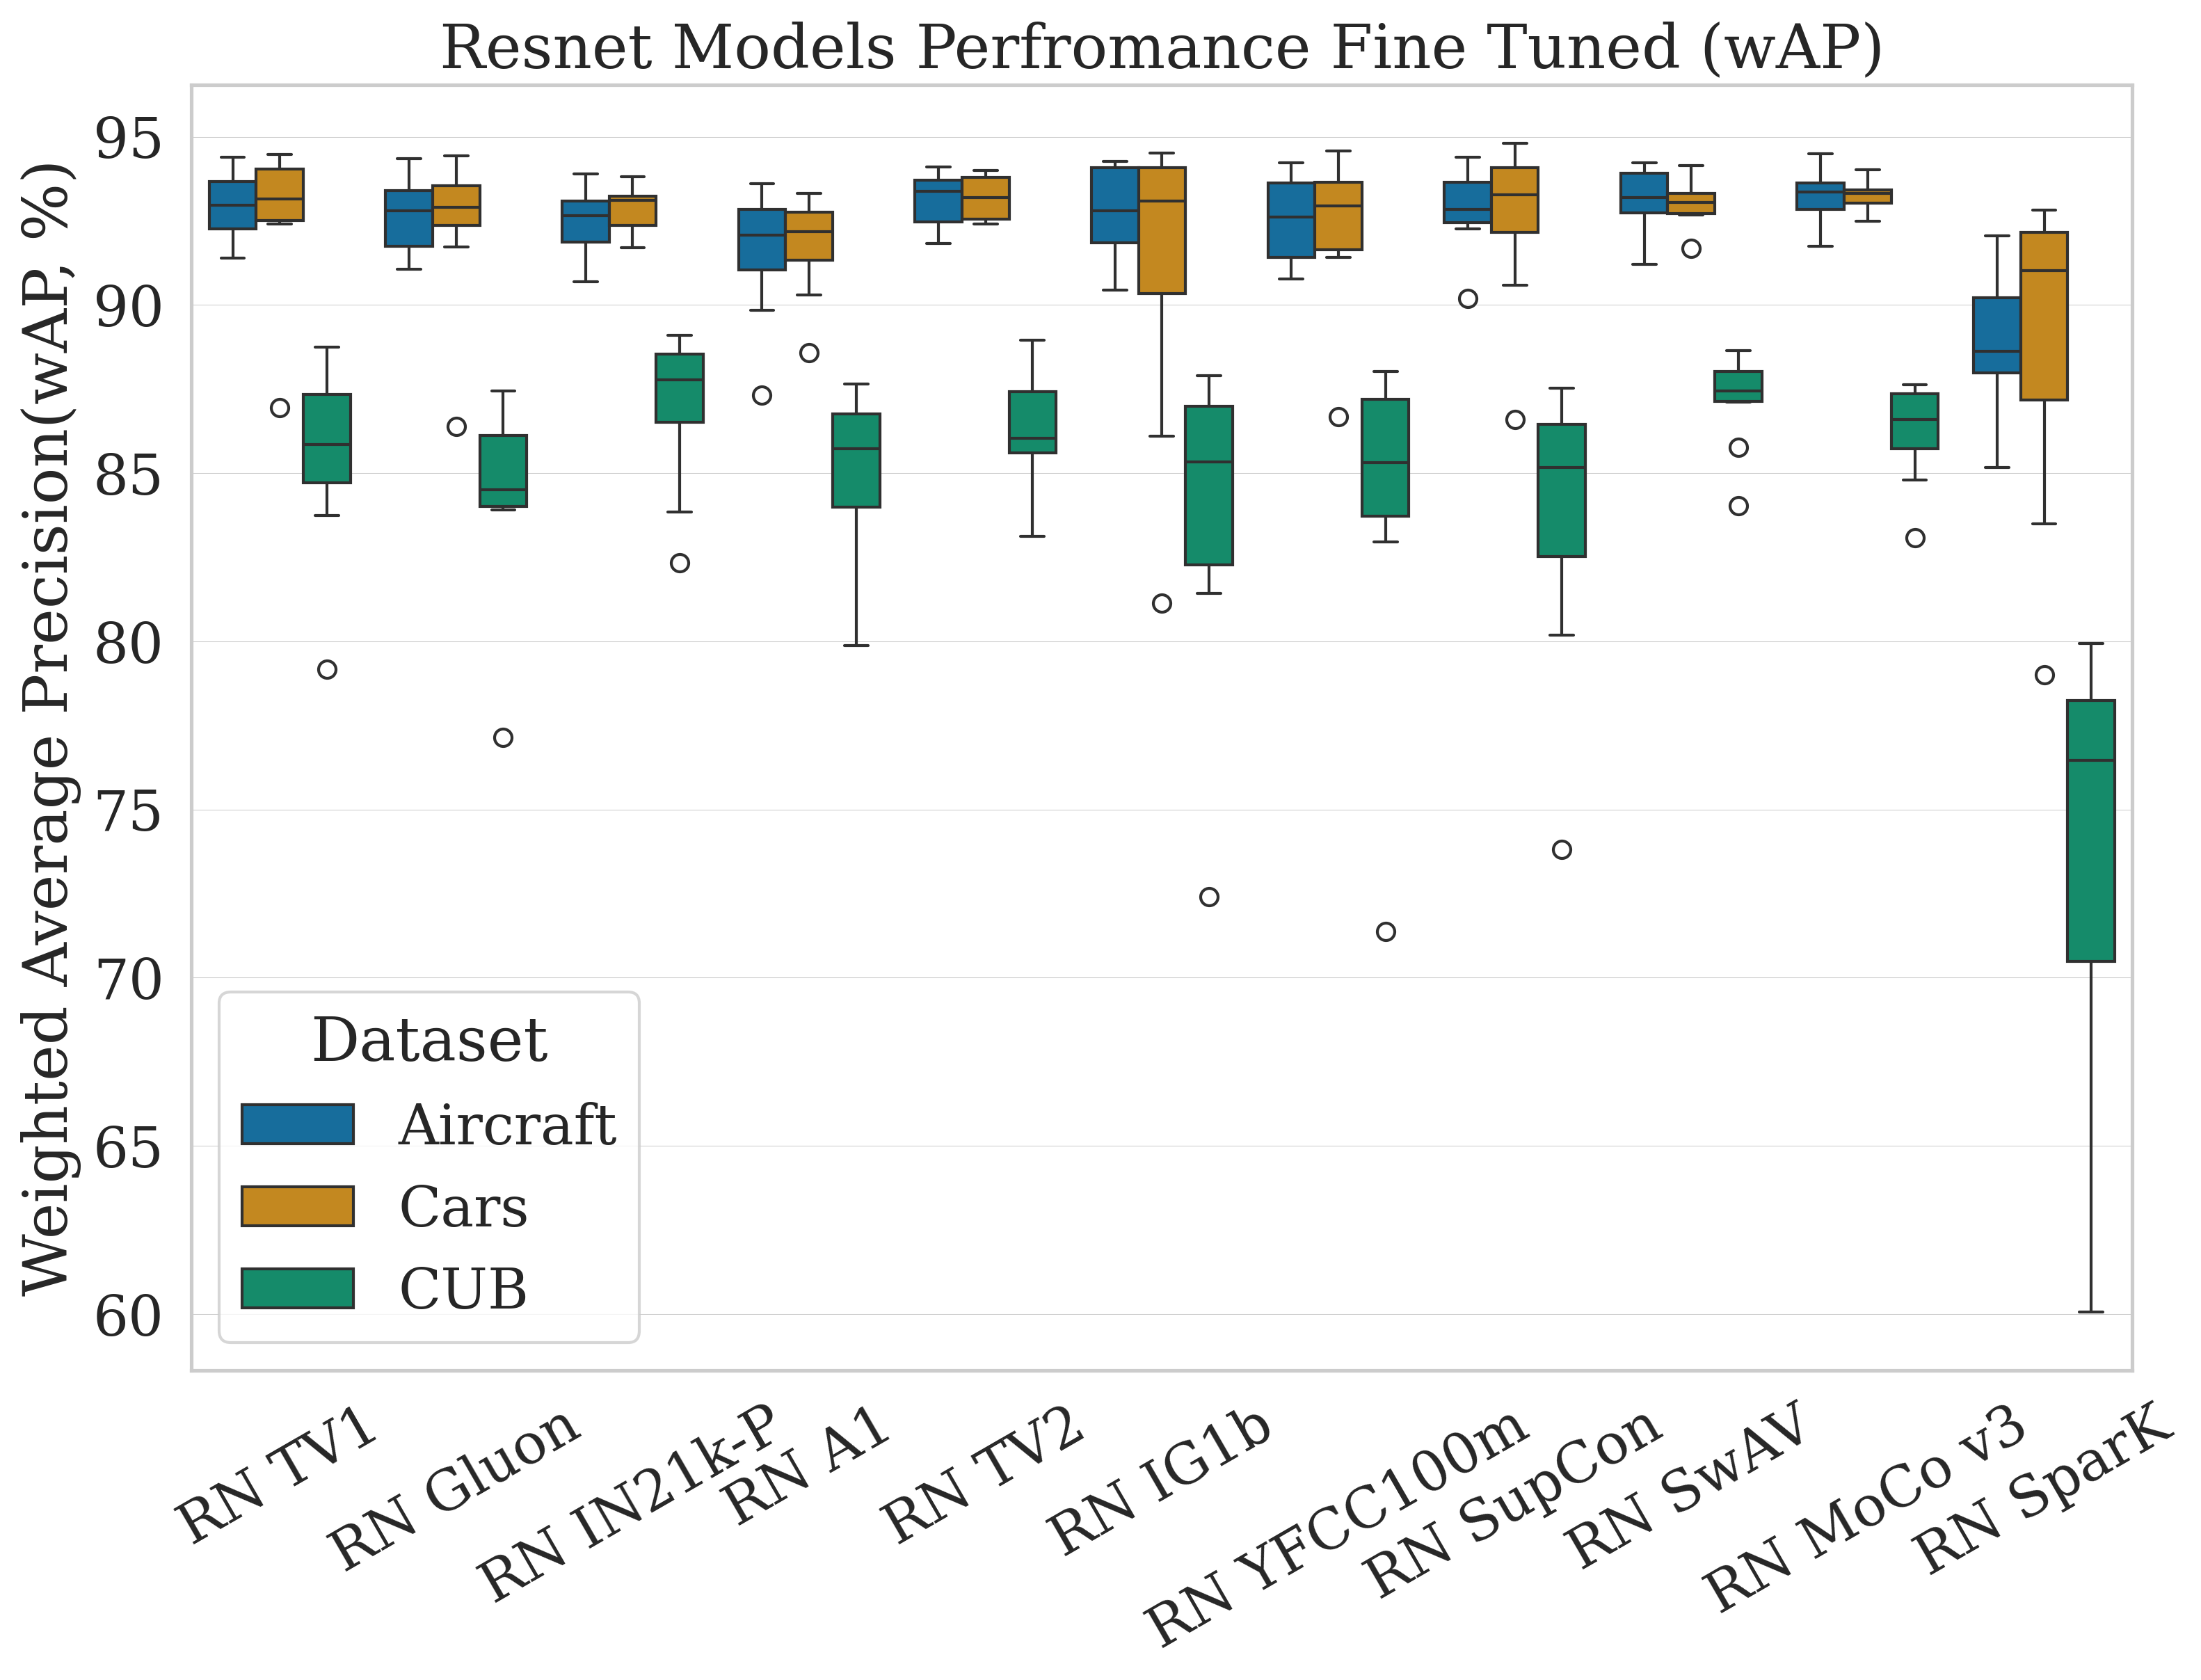
\includegraphics[width=\linewidth]{figures/rn_ft.png}
%         \label{fig_rn_ft}
%     \end{minipage}
%     \hspace{0.01\linewidth} 
%     \begin{minipage}{0.43\linewidth}
%         \centering
%         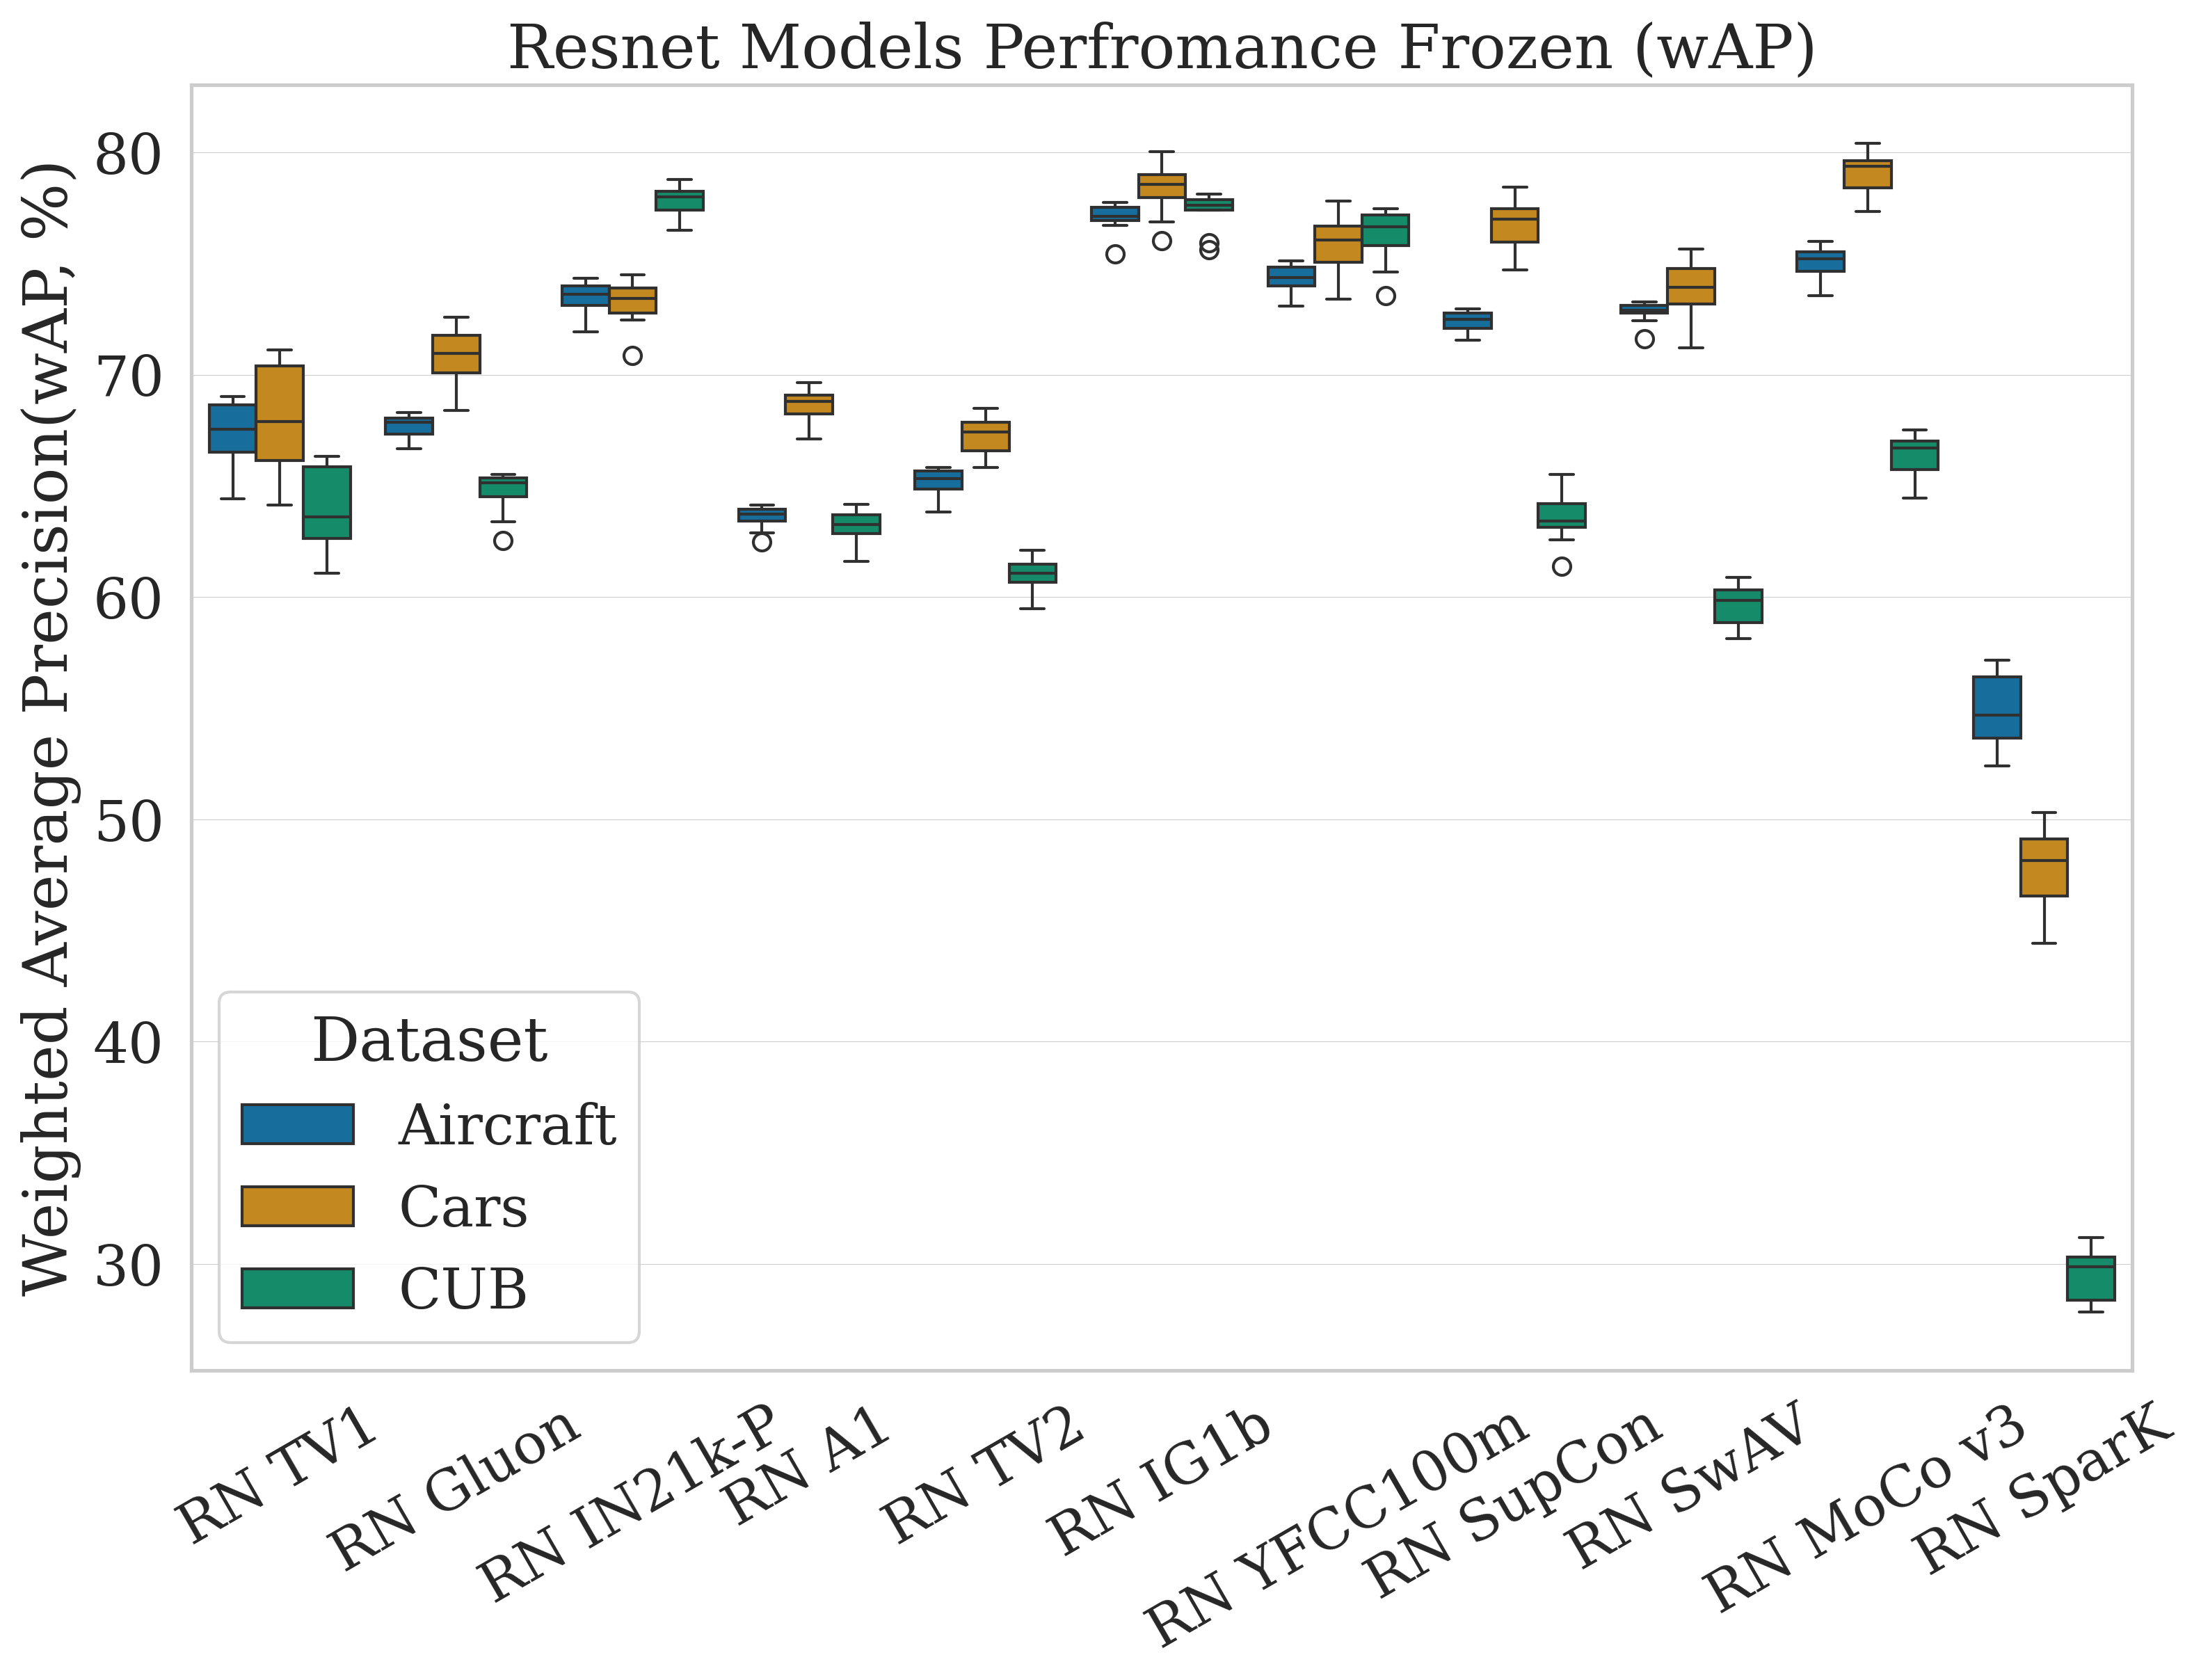
\includegraphics[width=\linewidth]{figures/rn_fz.png}
%         \label{fig_rn_fz}
%     \end{minipage}

%     \centering
%     \begin{minipage}{0.43\linewidth}
%         \centering
%         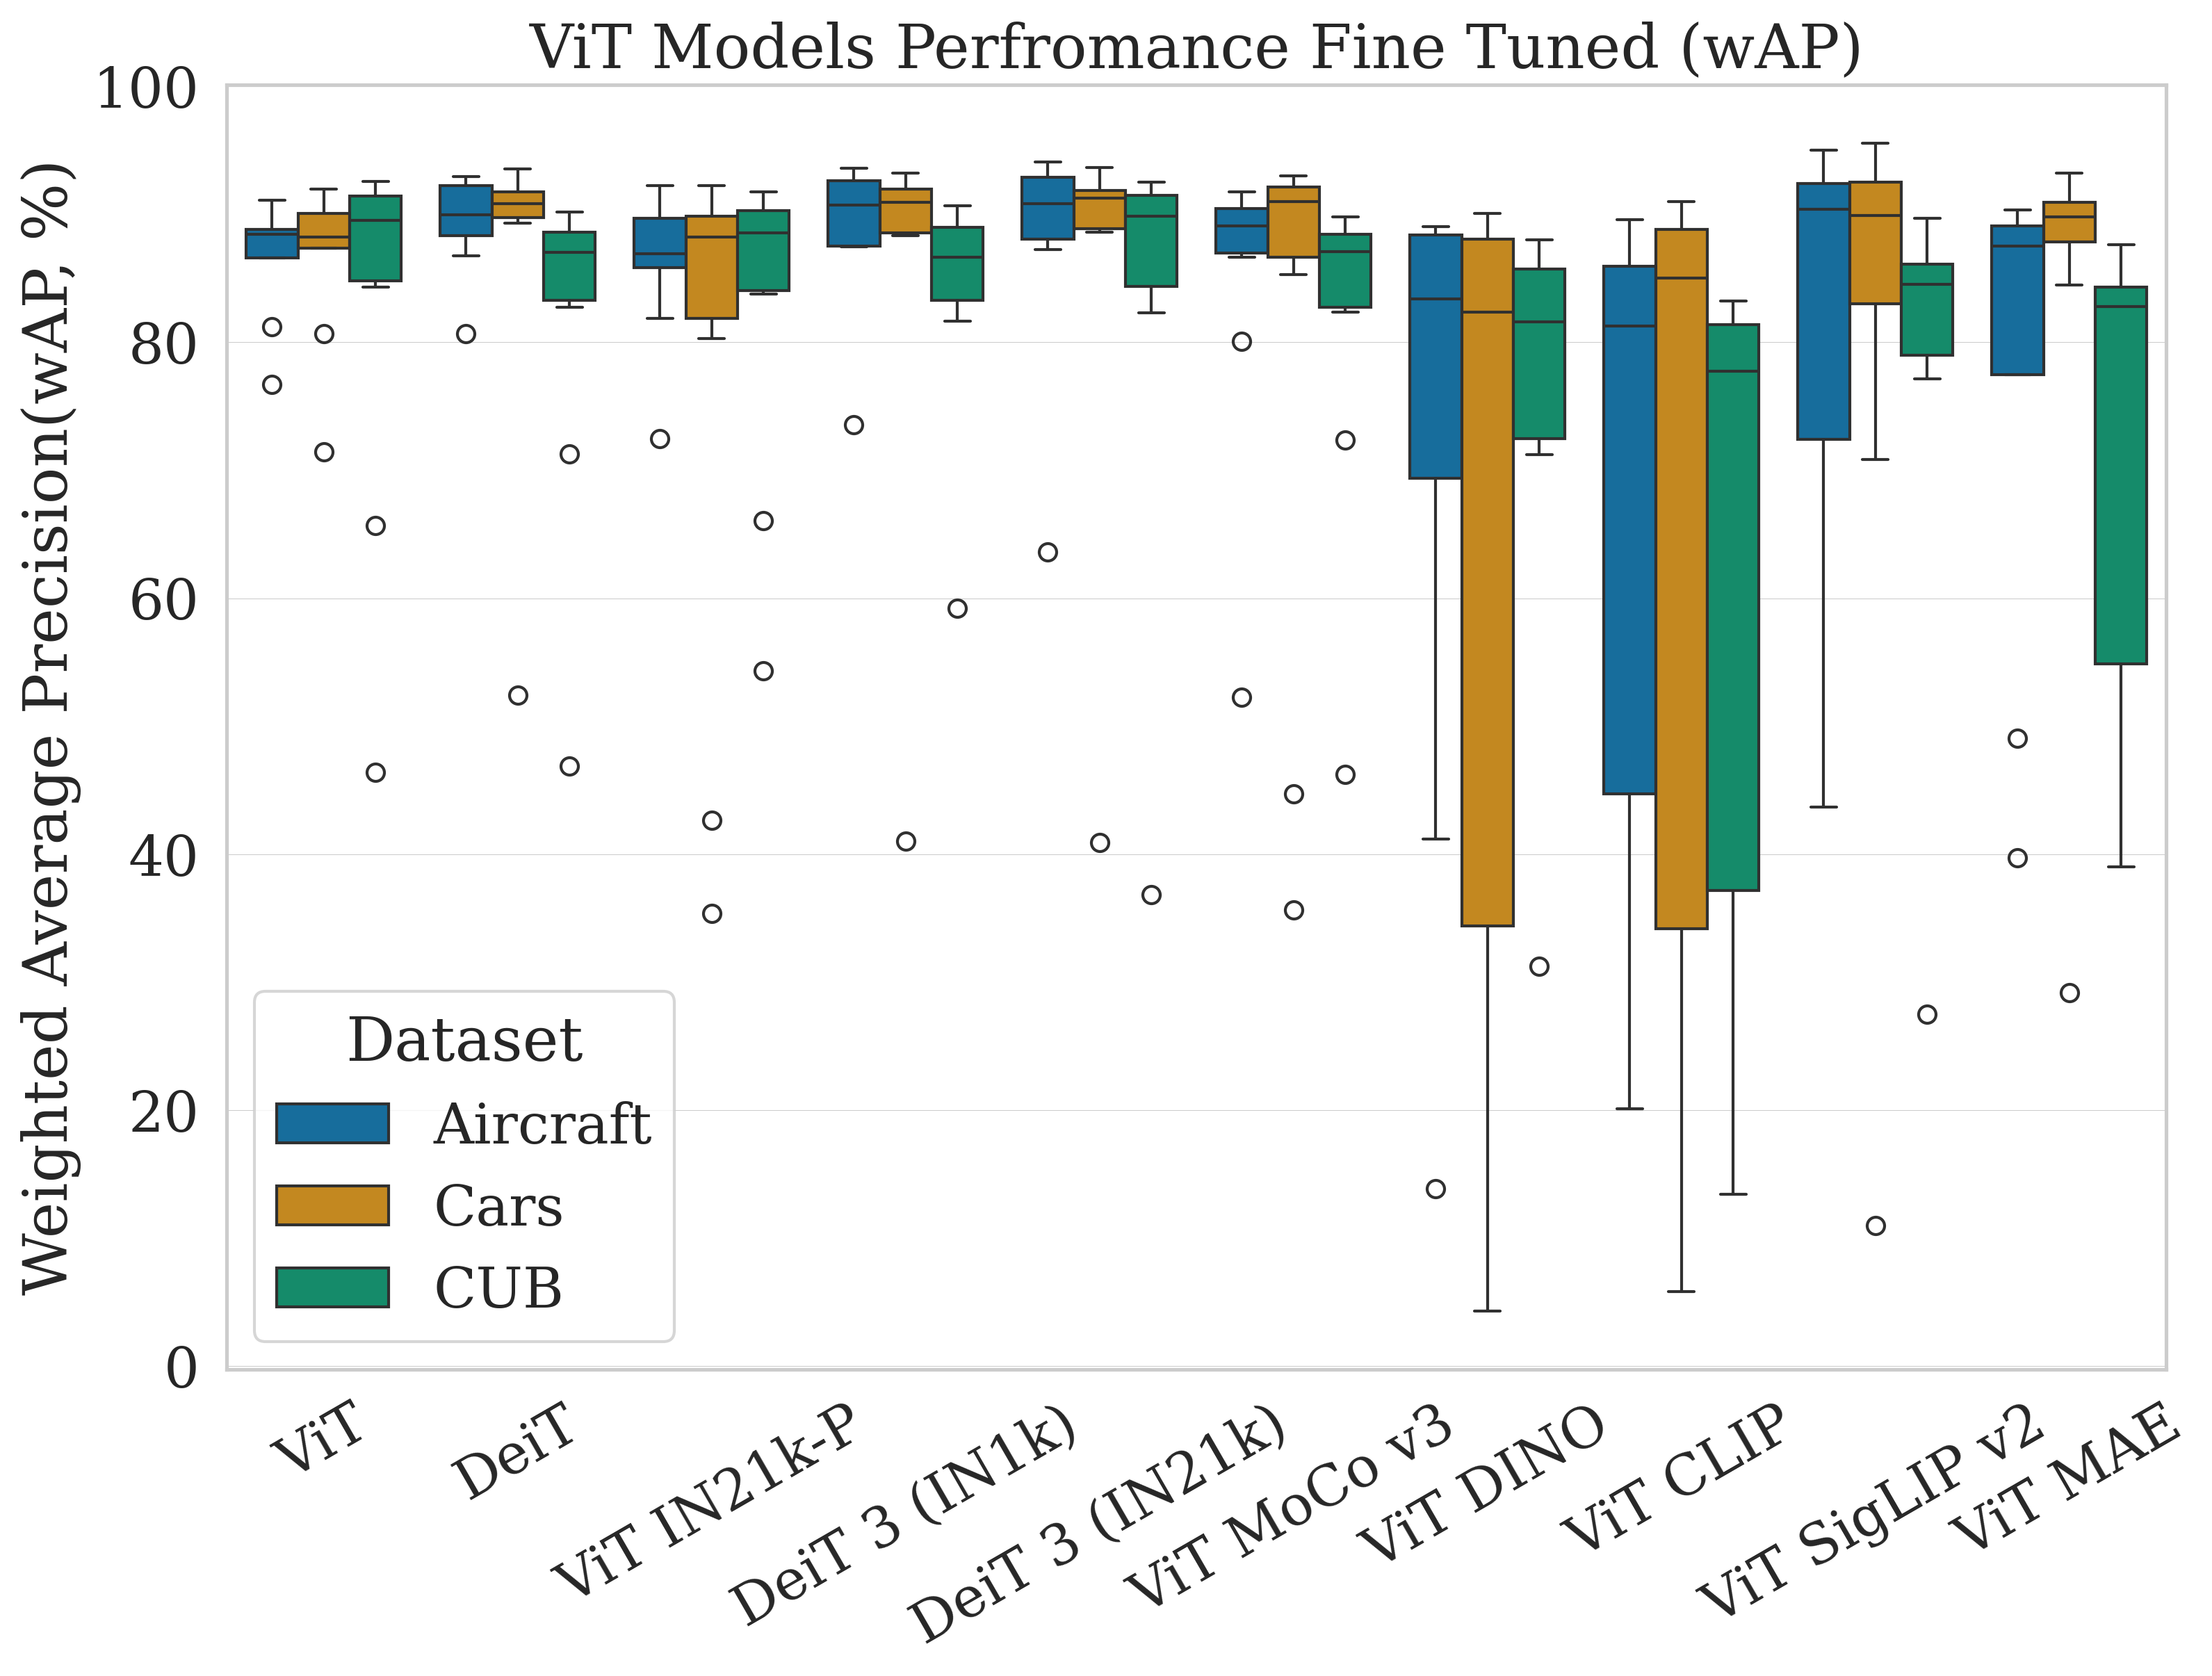
\includegraphics[width=\linewidth]{figures/vit_ft.png}
%         \label{fig_vit_ft}
%     \end{minipage}
%     \hspace{0.01\linewidth} 
%     \begin{minipage}{0.43\linewidth}
%         \centering
%         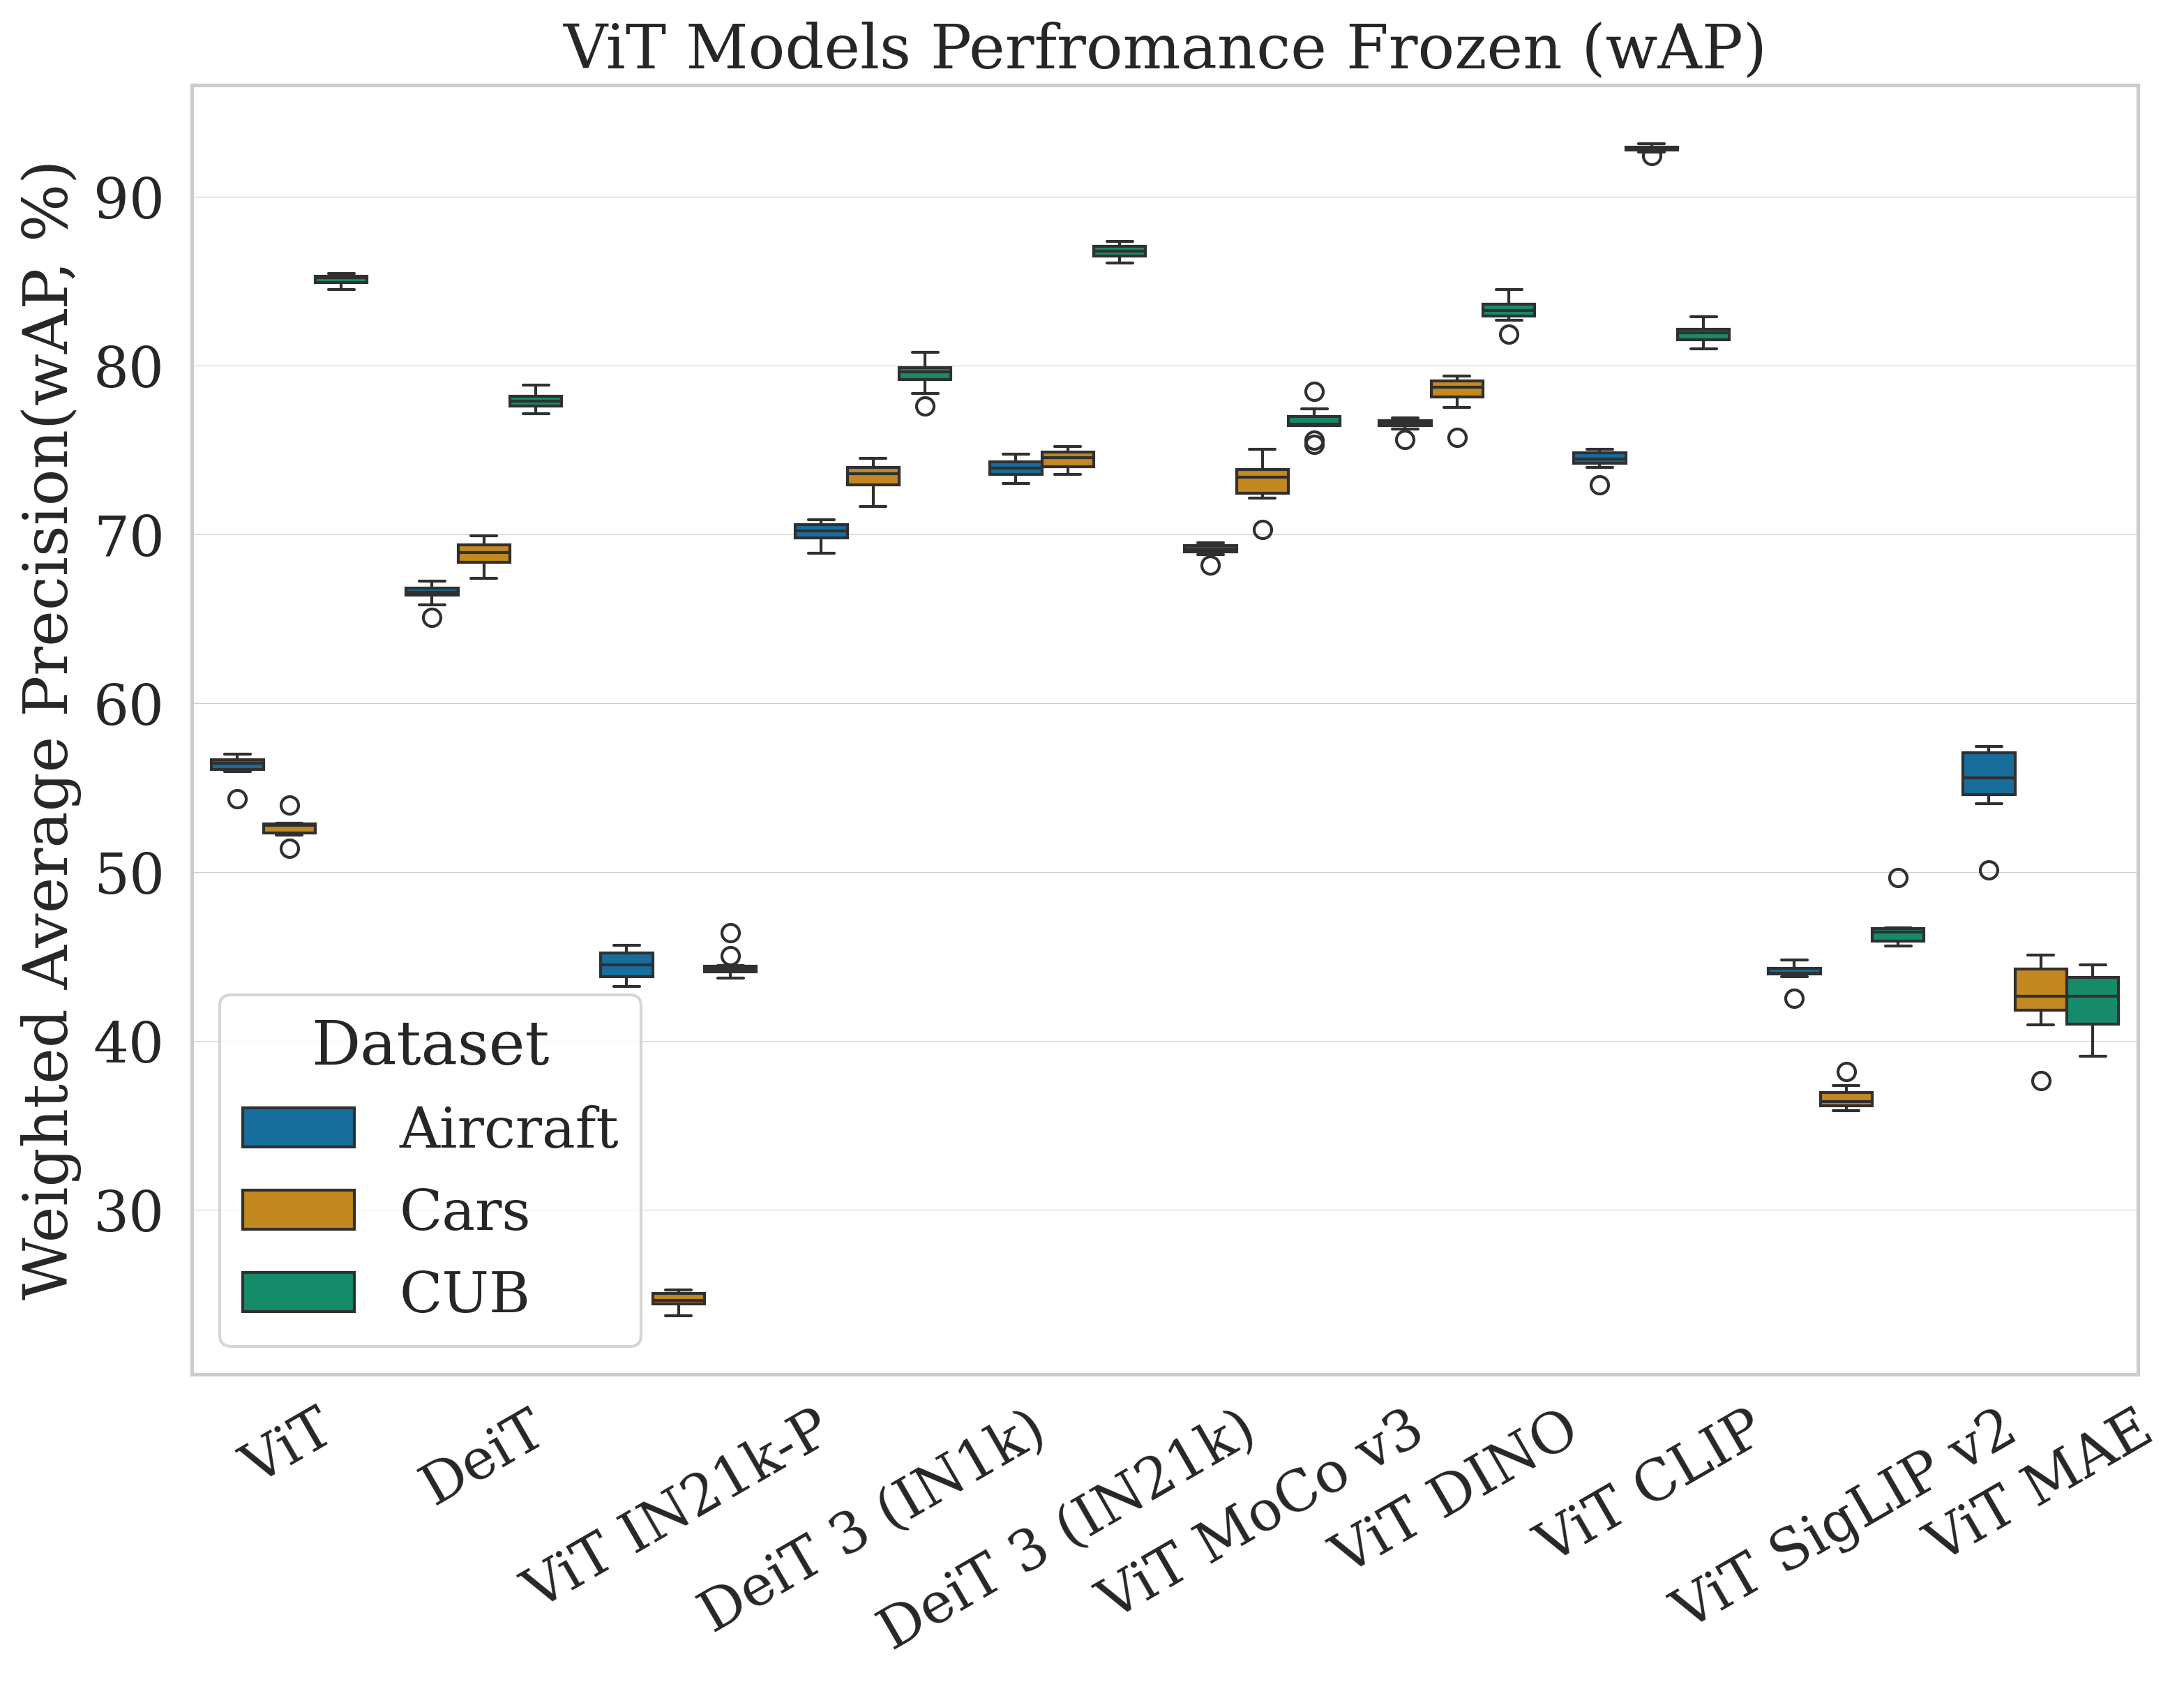
\includegraphics[width=\linewidth]{figures/vit_fz.png}
%         \label{fig_vit_fz}
%     \end{minipage}
%     \vspace{-0.55cm}
%     \caption{Backbone performance across training regimes. We compare ResNet (top) and ViT (bottom) models under fine-tuned (FT, left) and frozen (FZ, right) settings. Each plot shows the wAP performance distribution across models with different pretraining strategies.}
%     \label{fig_four_plot}
% \end{figure*}

\subsection{Impact of introducing Hierarchy on FGIR}
% \begin{table}[t]
% \centering
% \caption{ADA ratio across hyperparameters using RN IG1b as the evaluation backbone. Pseudo-hierarchies are constructed with two levels using either the same backbone (RN IG1b) or a stronger backbone (ViT SigLIP v2), with different coarse-label ratios. Lower is better.}
% \label{tab:baseline_vs_pseudohierarchy}
% \begin{tabularx}{\linewidth}{p{1.8615cm}XXXX}
% \toprule
% \multirow{2}{*}{Ratio (\%)} 
% & \multicolumn{2}{c}{Aircraft} 
% & \multicolumn{2}{c}{CUB} \\
% \cmidrule(lr){2-3} \cmidrule(lr){4-5}
% & IG1b
% & SigLiPv2
% & IG1b
% & SigLiPv2 \\
% \midrule
% No Hierarchy 
% & \multicolumn{2}{c}{3.08} 
% & \multicolumn{2}{c}{8.67} \\
% \midrule
% 10 & 1.77 & \underline{1.81} & \underline{7.25} & 9.34 \\
% 20 & 2.27 & \textbf{1.75} & 8.04 & 8.66 \\
% 30 & 1.71 & 1.82 & 7.32 & 7.43 \\
% 40 & 1.77 & 2.43 & \textbf{6.97} & 8.22 \\
% 50 & \underline{1.68} & 2.08 & 8.02 & \textbf{6.84} \\
% 70 & \textbf{1.54} & 1.92 & 8.59 & \underline{7.03} \\
% \bottomrule
% \end{tabularx}
% \end{table}

\subsubsection{Introducing hierarchy improves robustness}
Fig. \ref{fig_pseudo_main_rn} and  Fig. \ref{fig_pseudo_main_vit} show that hierarchical supervision consistently improves robustness across architectures, as indicated by lower CV compared to baseline. In ResNet models, hierarchy can reduce CV by almost half. For example, ResNet IG1b on Aircraft drops CV from 3.079 to 1.729, which is almost half. This effect is more pronounced for ViT models, which are more sensitive to hyperparameter choices. ViT base on Aircraft drops CV by nearly fourfold from 24.997 to 6.250.

\subsubsection{Hierarchy is more effective on machine-centric datasets}
\label{sec:hierarchy_machine_centric}
The impact of real hierarchical supervision varies across datasets, with larger CV reductions observed on Aircraft and Cars as shown in Fig. \ref{fig_pseudo_main_rn} and  Fig. \ref{fig_pseudo_main_vit}. For example, ResNet IG1b sees CV decrease from 3.079 to 1.729 on Aircraft and from 6.691 to 0.698 on Cars, whereas on CUB the reduction is smaller, from 7.035 to 6.191. This trend may reflect dataset-specific characteristics discussed in our backbone analysis \ref{sec:dataset_differences}, where more static shapes in Aircraft and Cars compared to more dynamic shapes in CUB, could influence the effectiveness of hierarchy in improving robustness.


\begin{figure*}[!htb]
    \centering
    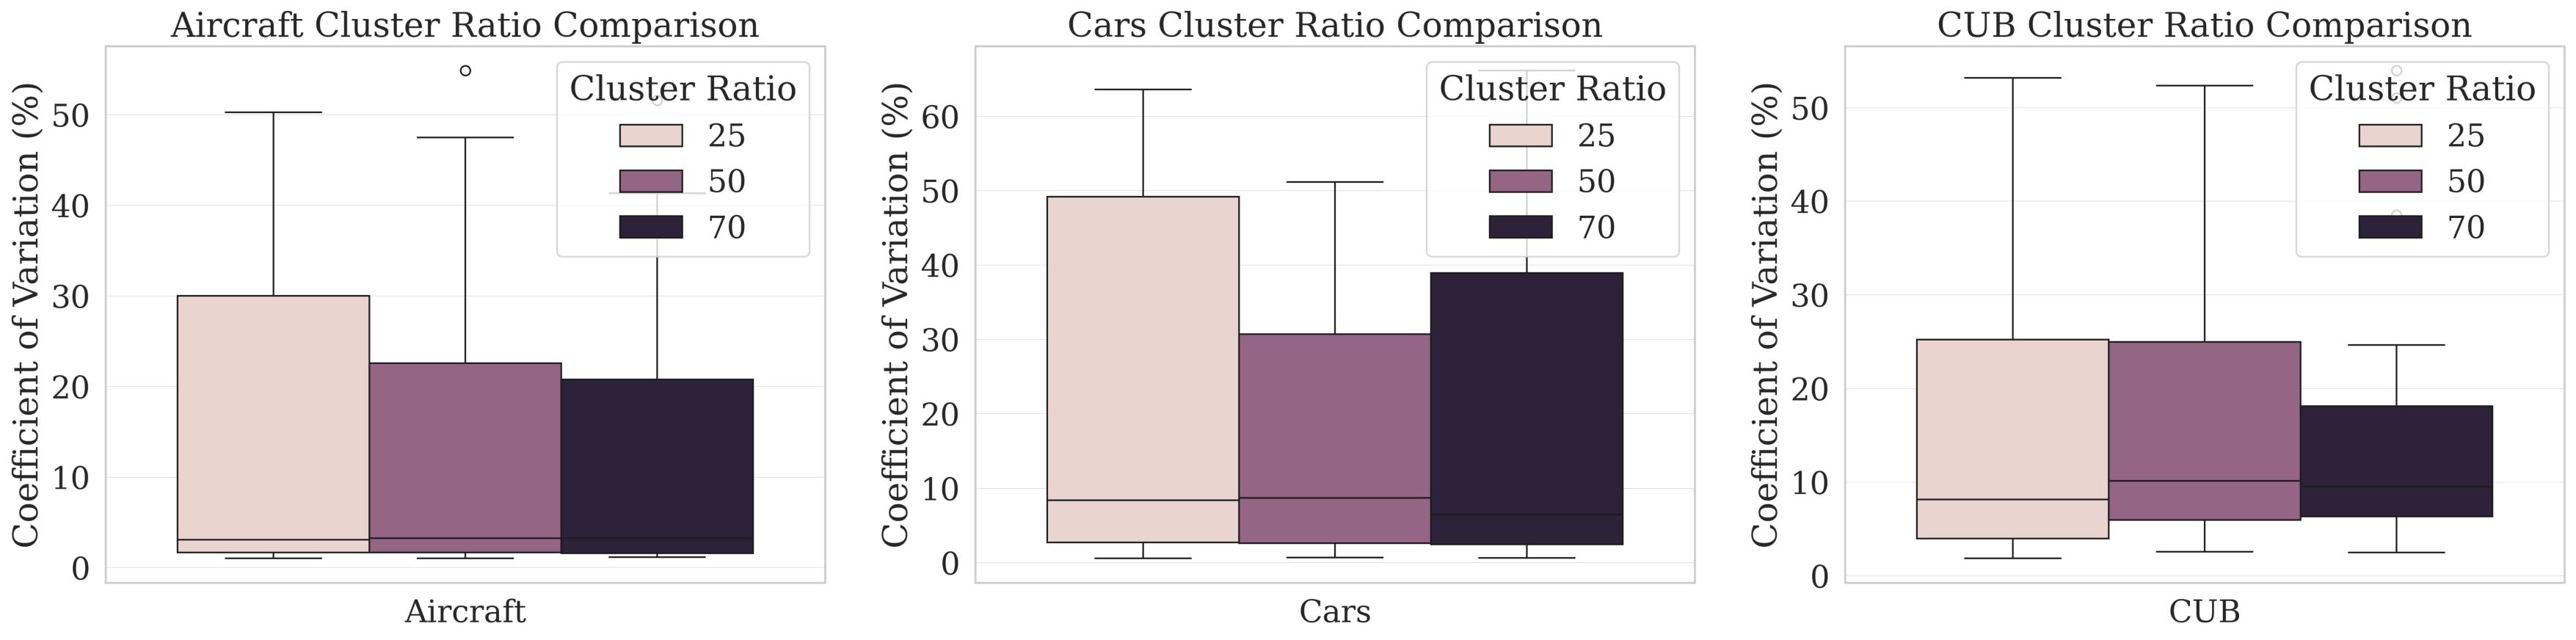
\includegraphics[width=0.75\textwidth]{figures/combined_ratio_plots.png}
    \caption{Coefficient of Variations (CV) across 3 different cluster ratio: 25\%, 50\%, and 70\% and 3 datasets. Lower is better.}
    \label{fig_pseudo_ratios}
\end{figure*}

\subsection{Pseudo-hierarchy on FGIR}
\subsubsection{Robustness improvements over Baseline}
Our pseudo-hierarchy method generally improves robustness of hyperparameter settings over baseline, as shown in Fig.\ref{fig_pseudo_main_rn} and Fig.\ref{fig_pseudo_main_vit}. The largest decreases in variance are observed for ViT backbones, such as MAE and SigLipv2, showing that pseudo-hierarchical clustering can stabilize predictions for models that are otherwise sensitive to hyperparameter choices. Across most models, the robustness gains from pseudo-hierarchies are comparable to those achieved with manually defined real hierarchies, and for some models, such as SigLipv2, pseudo-hierarchies even surpass the real hierarchy. These results demonstrate that pseudo-hierarchy offers a lightweight alternative to real hierarchical labels, improving model robustness across hyperparameters without the hefty cost of manual annotation.

\subsubsection{Pseudo-hierarchy impact on accuracy}
While pseudo-hierarchies generally improve robustness, their impact on mean accuracy is modest for most models. Across most of backbones, accuracy gains range from 1\% to 5\%, indicating that pseudo-hierarchy primarily stabilizes predictions rather than dramatically increasing overall performance. However, certain ViT backbones show substantial improvements: SigLipv2 gains up to 31.2\% accuracy increase, CLIP gains 34.3\%, and ViT MAE gains 51.8\%. Overall, these results show that while pseudo-hierarchies improve robustness, the corresponding gains in accuracy are smaller, barring a few exceptions.

\subsubsection{Impact on dataset group}
The impact of pseudo-hierarchies varies across datasets. On the machine-centric datasets, \textbf{FGVC Aircraft} and \textbf{Stanford Cars}, pseudo-hierarchy generally improves robustness compared to the baseline. Most backbones exhibit improved robustness across hyperparameter settings, indicating more stable training behavior. Only a few exceptions are observed among self-supervised models such as SwAV and SupCon. In contrast, the results on \textbf{CUB-200-2011} are more mixed. While some models still benefit from pseudo-hierarchies, many show robustness similar to the baseline, and a few backbones obtain worse robustness. Overall, the robustness improvements on CUB are smaller than those observed on Aircraft and Cars. This trend may reflect dataset-specific characteristics discussed in our backbone analysis \ref{sec:dataset_differences} and tied to section \ref{sec:hierarchy_machine_centric}, where more static shapes in Aircraft and Cars compared to more dynamic shapes in CUB, could influence the effectiveness of hierarchy in improving robustness.

\begin{figure*}[!htb]
    \centering
    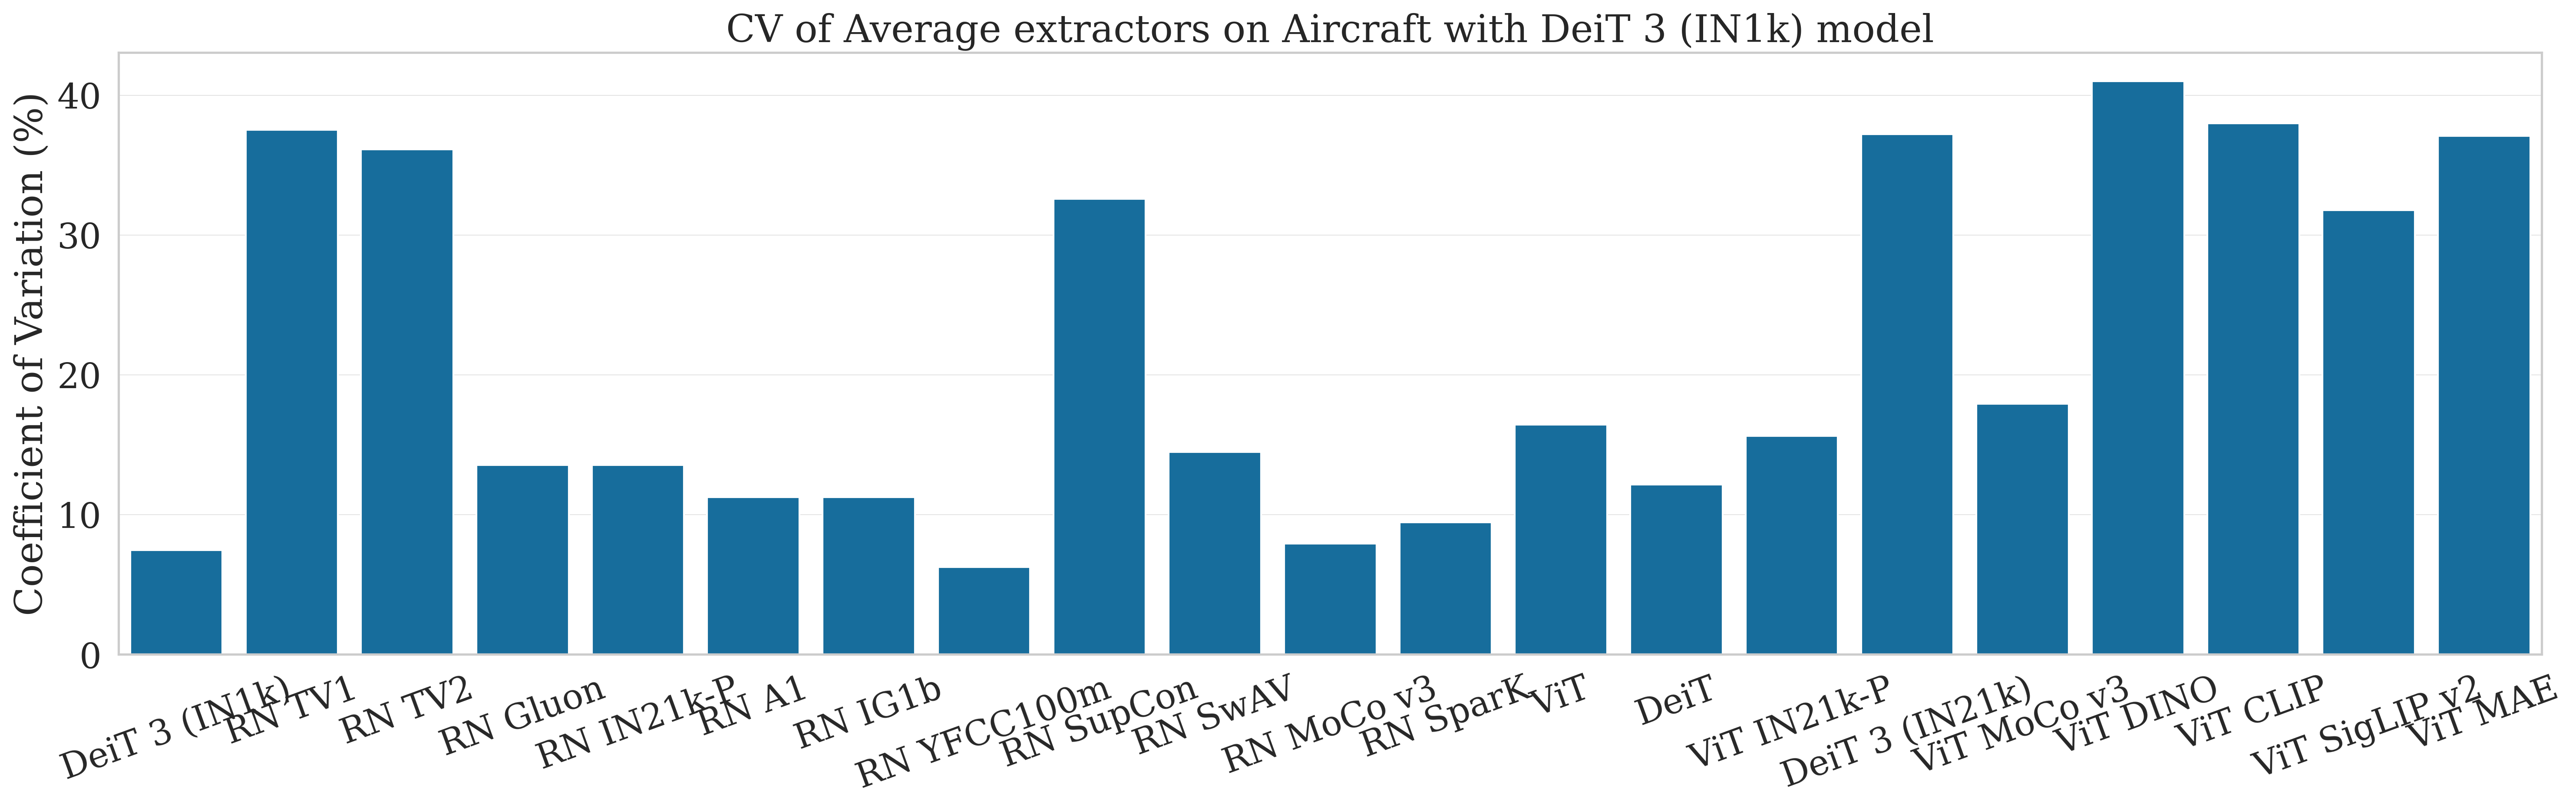
\includegraphics[width=0.75\textwidth]{figures/compare_extractors.png}
    \caption{Comparison of 21 feature extractor on Deit3 backbone on Aircraft measured using Coefficient of Variation (CV). Lower is better.}
    \label{fig_pseudo_extractor}
\end{figure*}

\section{Ablation Studies}
\subsection{Ablation on Cluster Ratios}
We evaluate three pseudo-hierarchy cluster ratios (25\%, 50\%, and 70\%) to analyze the impact of the number of coarse clusters on model robustness and performance. These results are shown in Fig.\ref{fig_pseudo_ratios}. Across all datasets, the 25\% ratio consistently obtains the highest CV. In contrast, ratios of 50\% and 70\% generally produce more stable results. For the Aircraft and CUB datasets, the 70\% ratio yields the lowest CV, while the Cars dataset yields the lowest CV with the 50\% ratio.

The inferior performance of lower cluster ratios may be attributed to the number of fine-grained classes in each dataset. Smaller ratios produce a relatively small number of coarse clusters. This can lead to overly broad groupings that dilute semantic similarity within clusters, reducing the effectiveness of the pseudo-hierarchy. Overall, these results indicate that higher cluster ratios (50\%–70\%) provide better pseudo-hierarchies, while small ratios, such as 25\% tend to degrade robustness.

\begin{figure}[ht]
    \centering
    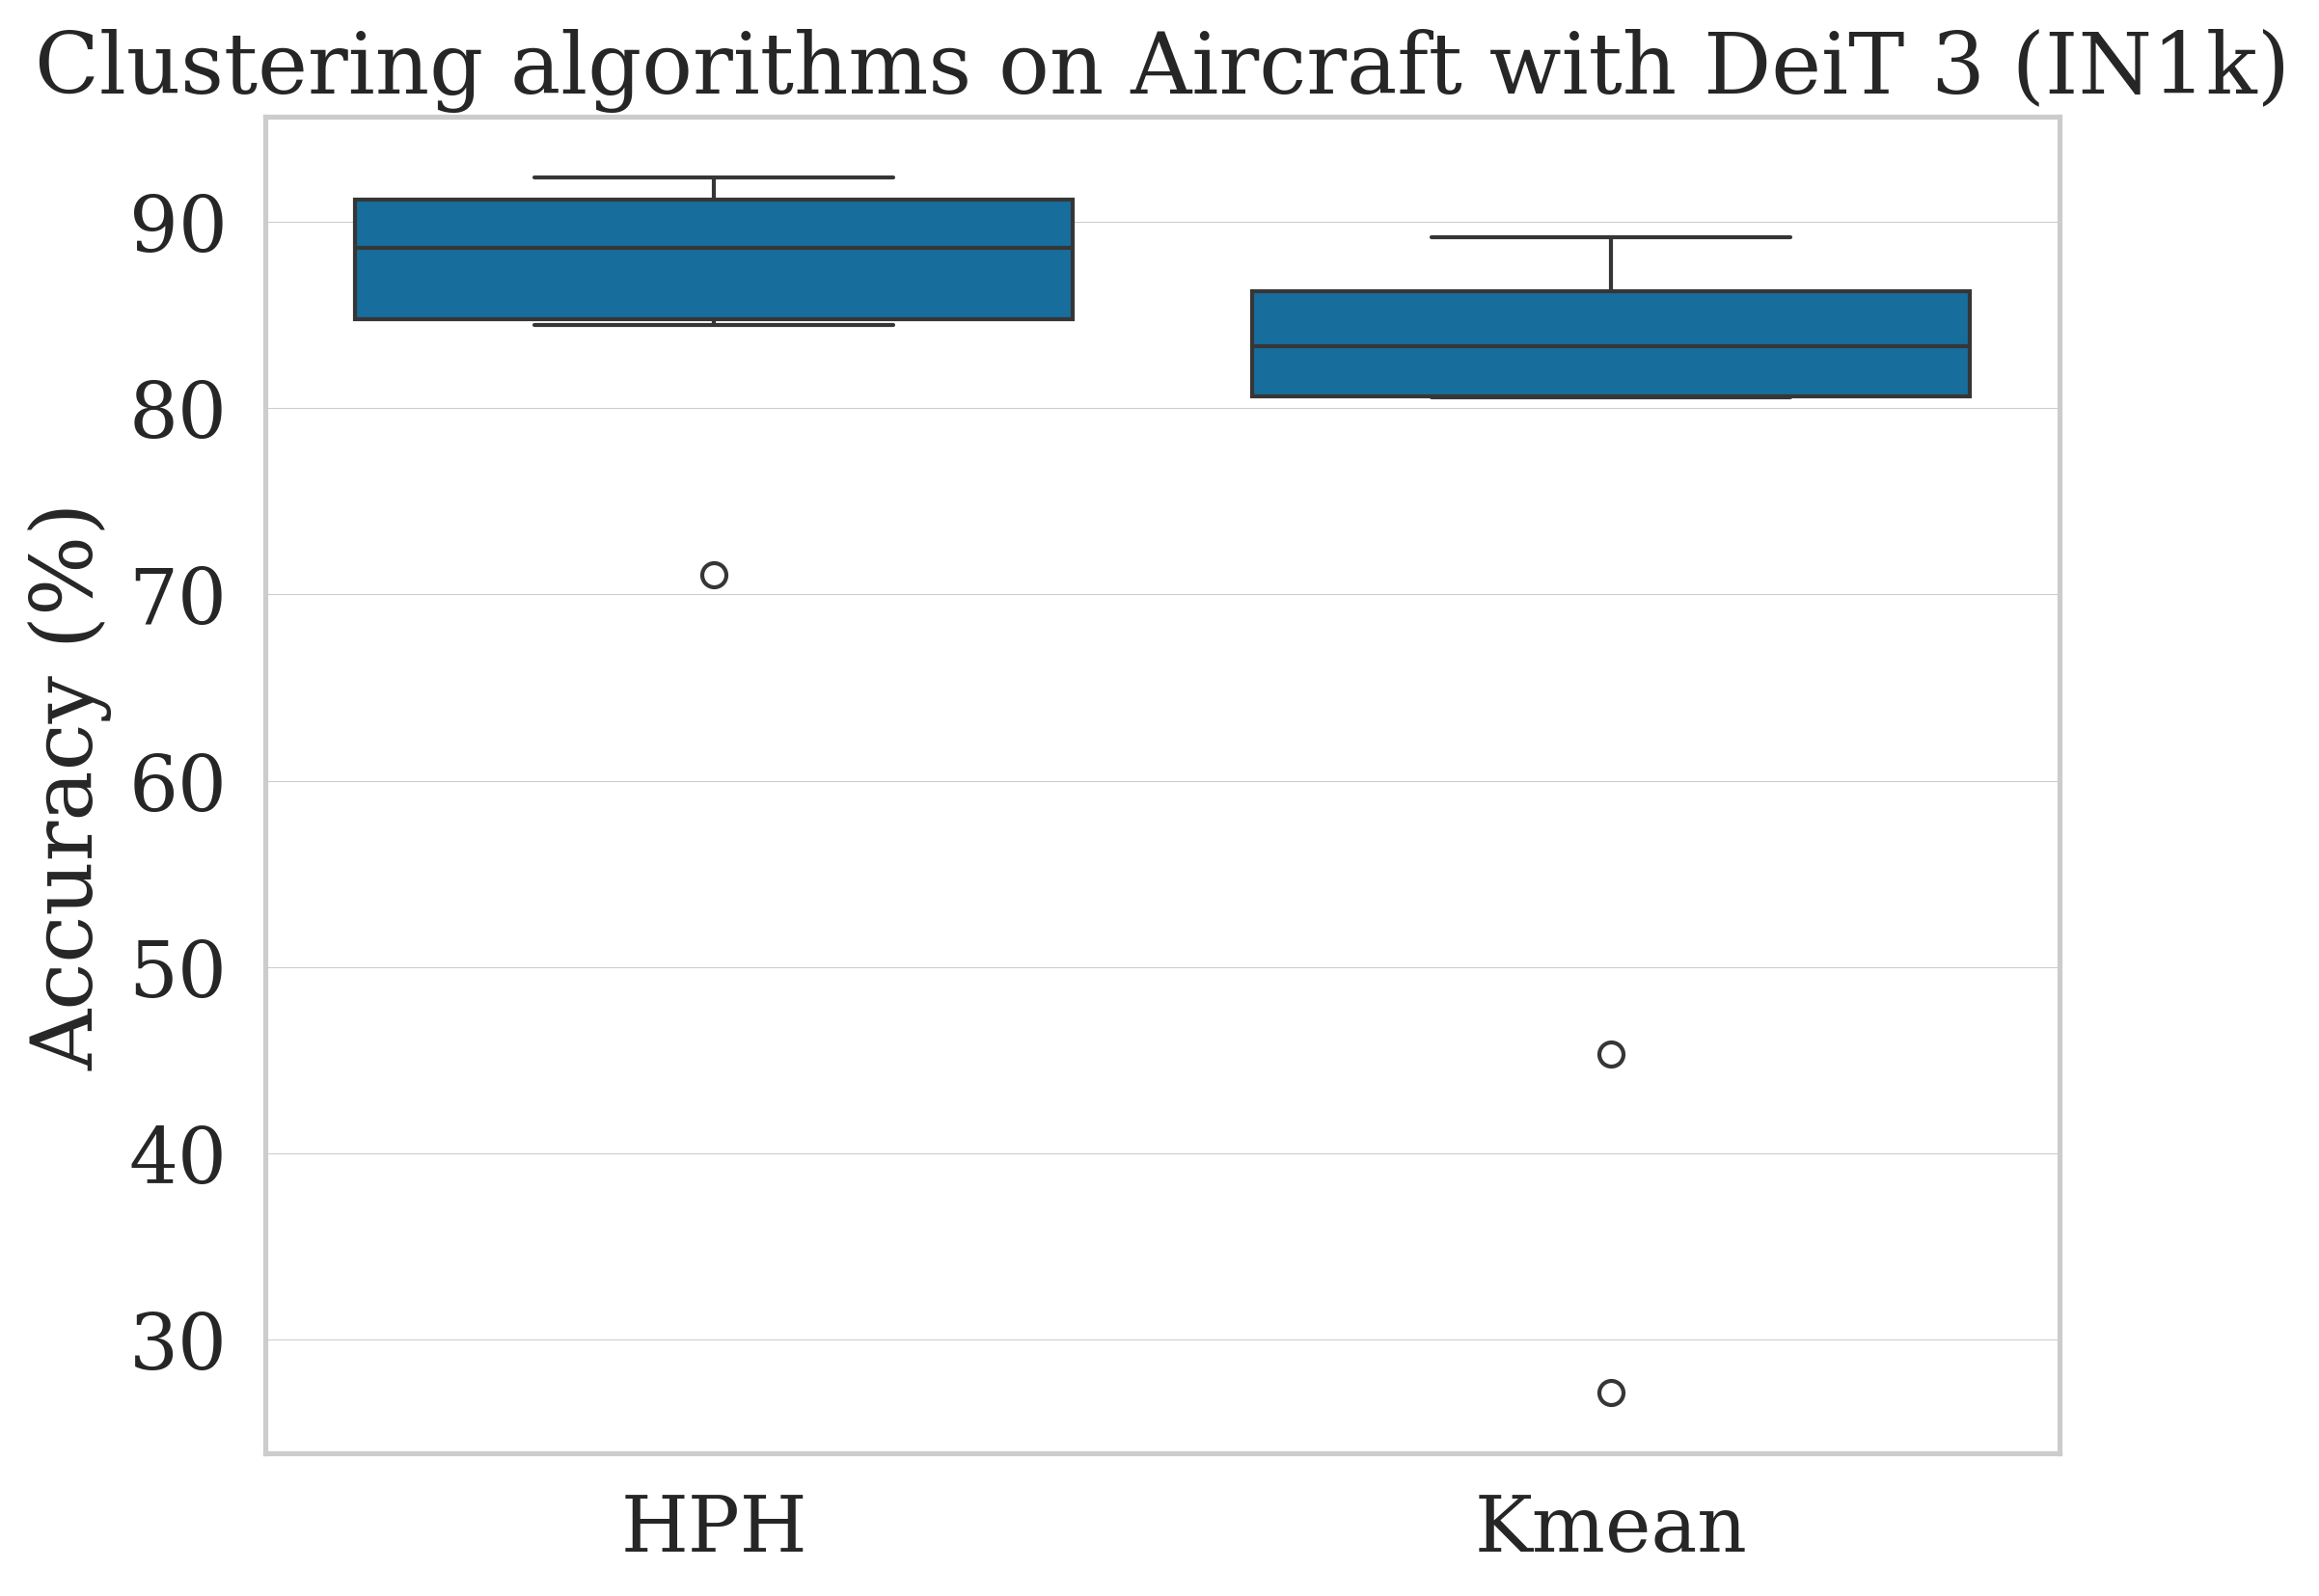
\includegraphics[width=0.75\linewidth]{figures/compare_algo.png}
    \caption{Comparison of Performance between our algorithm: Hungarian Pseudo-Hierarchy (HPH) vs other clustering algorithm.}
    \label{fig_pseudo_algo}
\end{figure}

\subsection{Ablation on Other Clustering Algorithm}
We compare our proposed pseudo-hierarchy construction with a commonly used clustering baseline, K-Means, on Aircraft with ViT Deit3 backbone as shown in Fig.\ref{fig_pseudo_algo}. Our method consistently obtains higher accuracy than K-Means, indicating improved robustness while also obtaining better accuracy. This result highlights the importance of the clustering strategy used to construct pseudo-hierarchies. Suboptimal cluster assignments may degrade both performance and robustness, while our proposed bipartite matching produces more stable hierarchical groupings, leading to improved overall performance of the hierarchical classifier.

\begin{figure}[ht]
    \centering
    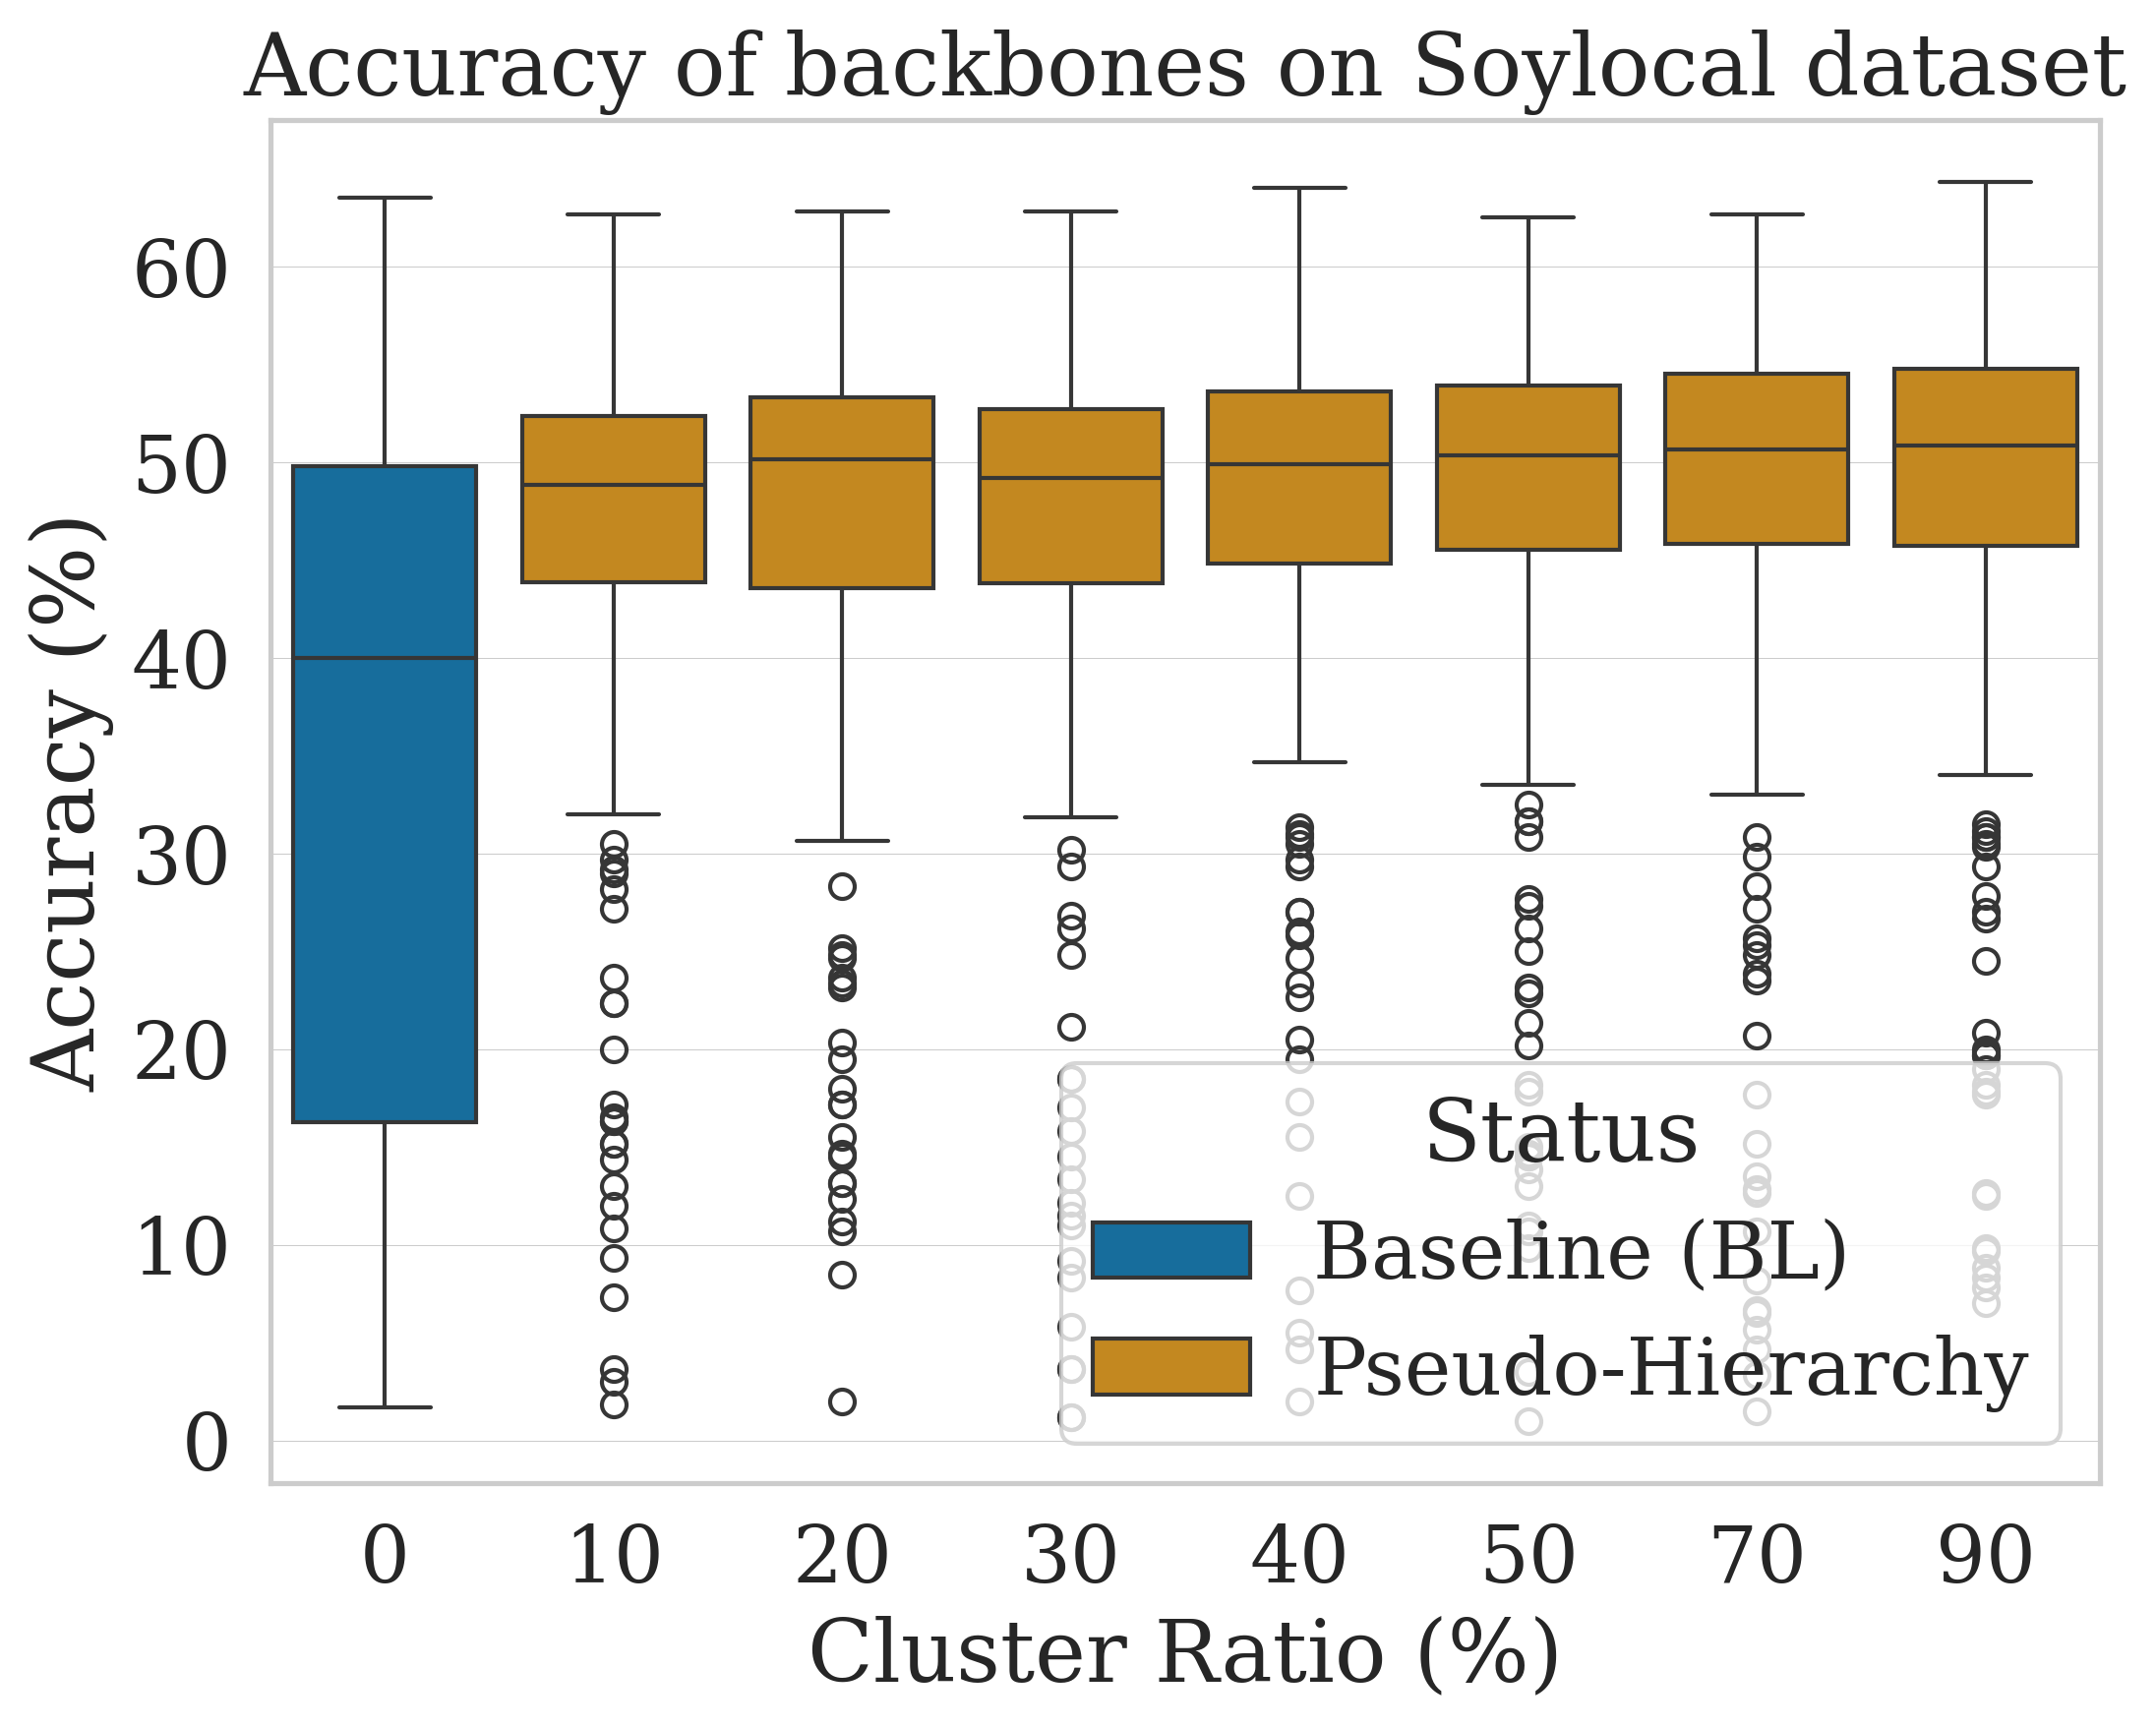
\includegraphics[width=0.75\linewidth]{figures/compare_soylocal.png}
    \caption{Comparison of 21 backbones on Soylocal dataset. Our method consistently obtains higher accuracy.}
    \label{fig_pseudo_soylocal}
\end{figure}

\subsection{Ablation on Other Datasets}
To evaluate whether our approach generalizes beyond the primary dataset, we conduct experiments on the SoyLocal dataset. SoyLocal is an Ultra Fine-Grained Image Recognition (UFGIR) dataset consisting of high-resolution soybean leaf images, containing 600 images across 200 fine-grained classes. Due to the extremely small number of samples per class, the dataset presents a challenging setting of unstable training. Fig.\ref{fig_pseudo_soylocal} shows the results of our pseudo-hierarchy approach across different clustering ratios (10, 20, 30, 40, 50, 70, and 90\%). Across all ratios, the pseudo-hierarchy consistently achieves higher classification mean accuracy and lower variance compared to the baseline.

\begin{figure}[ht]
    \centering
    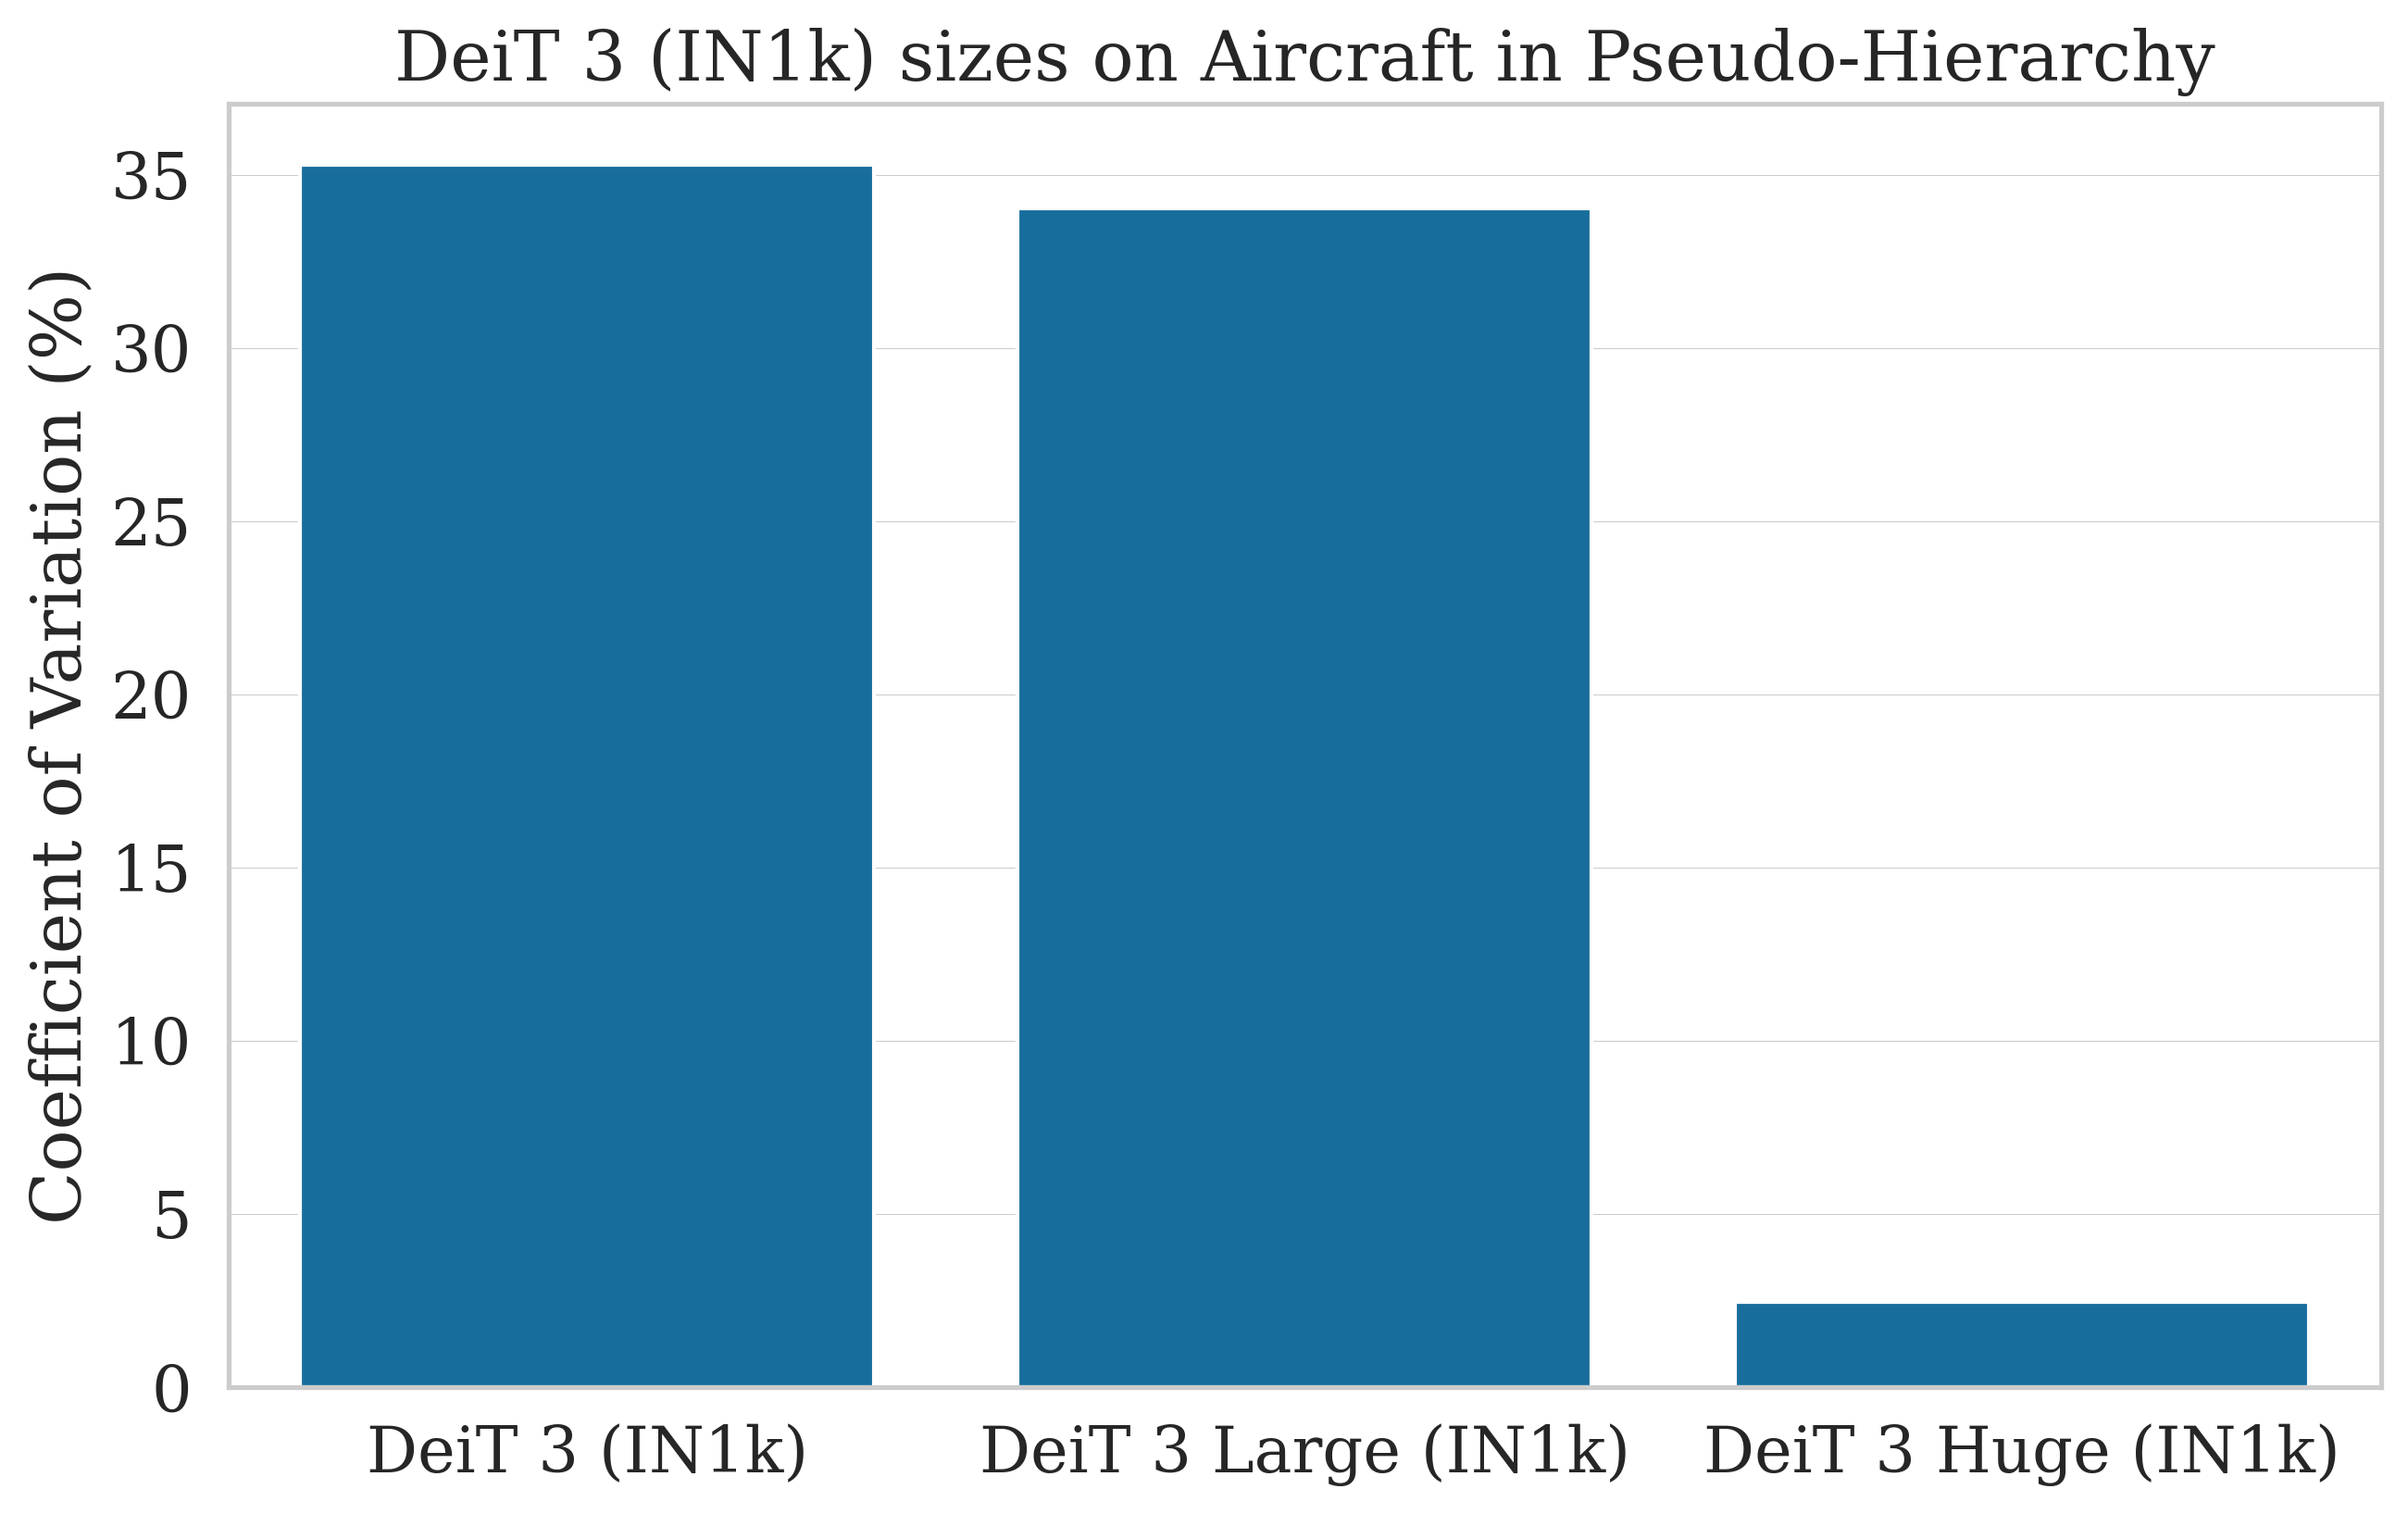
\includegraphics[width=0.75\linewidth]{figures/compare_model_size.png}
    \caption{Comparison of Deit3 backbone sizes on Aircraft measured using Coefficient of Variation (CV). Lower is better.}
    \label{fig_pseudo_model_size}
\end{figure}

\subsection{Ablation on Backbone Size}
We analyze the impact of backbone capacity by evaluating three model sizes from the DeiT3 family: Base, Large, and Huge. As shown in Fig.~\ref{fig_pseudo_model_size}, increasing the backbone size generally improves robustness under pseudo-hierarchical supervision. The DeiT3-Large model achieves a modest reduction in the Coefficient of Variation (CV) compared to DeiT3-Base, while DeiT3-Huge produces a substantially larger reduction in CV. This trend indicates that larger models benefit more strongly from the pseudo-hierarchical structure, likely due to their increased representational capacity. Overall, these results suggest that pseudo-hierarchy becomes increasingly effective as backbone capacity grows, providing stronger robustness improvements for larger models.

\subsection{Ablation on Different Extractors}
We further analyze the impact of feature extractor choice when constructing pseudo-hierarchies. Using DeiT3 as the training backbone on the Aircraft dataset, we evaluated 21 different pretrained backbones as feature extractors for clustering. The results are shown in Fig.~\ref{fig_pseudo_extractor}. Among the evaluated extractors, RN YFCC100M and the training backbone itself, DeiT3 (IN1K), produce some of the lowest CV, indicating stronger robustness compared to other feature extractors. These results suggest that strong pretrained representations are important for reliable pseudo-hierarchy construction. In practice, using the same backbone for feature extraction and training can serve as a simple and effective choice without requiring additional specialized extractors.

% \begin{abstract}
The ABSTRACT is to be in fully justified italicized text, at the top of the left-hand column, below the author and affiliation information.
Use the word ``Abstract'' as the title, in 12-point Times, boldface type, centered relative to the column, initially capitalized.
The abstract is to be in 10-point, single-spaced type.
Leave two blank lines after the Abstract, then begin the main text.
Look at previous \confName abstracts to get a feel for style and length.
\end{abstract}    
% \section{Introduction}
\label{sec:intro}

Please follow the steps outlined below when submitting your manuscript to the IEEE Computer Society Press.
This style guide now has several important modifications (for example, you are no longer warned against the use of sticky tape to attach your artwork to the paper), so all authors should read this new version.

%-------------------------------------------------------------------------
\subsection{Language}

All manuscripts must be in English.

\subsection{Dual submission}

Please refer to the author guidelines on the \confName\ \confYear\ web page for a
discussion of the policy on dual submissions.

\subsection{Paper length}
Papers, excluding the references section, must be no longer than eight pages in length.
The references section will not be included in the page count, and there is no limit on the length of the references section.
For example, a paper of eight pages with two pages of references would have a total length of 10 pages.
{\bf There will be no extra page charges for \confName\ \confYear.}

Overlength papers will simply not be reviewed.
This includes papers where margins and formatting are deemed to have been significantly altered from those laid down by this style guide.
Note that this \LaTeX\ guide already sets the figure captions and references in a smaller font.
The reason why such papers will not be reviewed is that there is no provision for supervised revisions of manuscripts.
The review process cannot determine the suitability of the paper for presentation in eight pages if it is reviewed in 11 pages.

%-------------------------------------------------------------------------
\subsection{The ruler}
The \LaTeX\ style defines a printed ruler that should be present in the version submitted for review.
The ruler is provided in order that reviewers may comment on particular lines in the paper without circumlocution.
If you are preparing a document using a non-\LaTeX\ document preparation system, arrange for an equivalent ruler to appear on the final output pages.
The presence or absence of the ruler should not change the appearance of any other content on the page.
The camera-ready copy should not contain a ruler.
(\LaTeX\ users may use the options of \texttt{cvpr.sty} to switch between different versions.)

Reviewers:
note that the ruler measurements do not align well with lines in the paper --- this turns out to be very difficult to do well when the paper contains many figures and equations, and, when done, looks ugly.
Use fractional references (\eg, this line is $087.5$), although in most cases the approximate location would be adequate.


\subsection{Paper ID}
Make sure that the Paper ID from the submission system is visible in the version submitted for review (replacing the ``*****'' you see in this document).
If you are using the \LaTeX\ template, \textbf{make sure to update paper ID in the appropriate place in the tex file}.


\subsection{Mathematics}

Please, number all of your sections and displayed equations as in these examples:
\begin{equation}
  E = m\cdot c^2
  \label{eq:important}
\end{equation}
and
\begin{equation}
  v = a\cdot t.
  \label{eq:also-important}
\end{equation}
It is important for the reader to be able to refer to any particular equation.
Just because you did not refer to it in the text does not mean that some future reader might not need to refer to it.
It is cumbersome to have to use circumlocutions like ``the equation second from the top of page 3 column 1''.
(Note that the ruler will not be present in the final copy, so is not an alternative to equation numbers).
All authors will benefit from reading Mermin's description of how to write mathematics:
\url{http://www.pamitc.org/documents/mermin.pdf}.

\subsection{Blind review}

Many authors misunderstand the concept of anonymizing for blind review.
Blind review does not mean that one must remove citations to one's own work---in fact it is often impossible to review a paper unless the previous citations are known and available.

Blind review means that you do not use the words ``my'' or ``our'' when citing previous work.
That is all.
(But see below for tech reports.)

Saying ``this builds on the work of Lucy Smith [1]'' does not mean that you are Lucy Smith;
it says that you are building on her work.
If you are Smith and Jones, do not say ``as we show in [7]'', say ``as Smith and Jones show in [7]'' and at the end of the paper, include reference 7 as you would any other cited work.

An example of a bad paper just asking to be rejected:
\begin{quote}
\begin{center}
    An analysis of the frobnicatable foo filter.
\end{center}

   In this paper, we present a performance analysis of our previous paper [1], and show that it is inferior to all previously known methods.
   Why the previous paper was accepted without this analysis is beyond me.

   [1] Removed for blind review
\end{quote}


An example of an acceptable paper:
\begin{quote}
\begin{center}
     An analysis of the frobnicatable foo filter.
\end{center}

   In this paper, we present a performance analysis of the paper of Smith \etal [1], and show it to be inferior to all previously known methods.
   Why the previous paper was accepted without this analysis is beyond me.

   [1] Smith, L and Jones, C. ``The frobnicatable foo filter, a fundamental contribution to human knowledge''. Nature 381(12), 1-213.
\end{quote}

If you are making a submission to another conference at the same time that covers similar or overlapping material, you may need to refer to that submission to explain the differences, just as you would if you had previously published related work.
In such cases, include the anonymized parallel submission~\cite{Authors14} as supplemental material and cite it as
\begin{quote}
[1] Authors. ``The frobnicatable foo filter'', F\&G 2014 Submission ID 324, Supplied as supplemental material {\tt fg324.pdf}.
\end{quote}

Finally, you may feel you need to tell the reader that more details can be found elsewhere and refer them to a technical report.
For conference submissions, the paper must stand on its own, and not {\em require} the reviewer to go to a tech report for further details.
Thus, you may say in the body of the paper ``further details may be found in~\cite{Authors14b}''.
Then submit the tech report as supplemental material.
Again, do not assume that the reviewers will read this material.

Sometimes your paper is about a problem that you tested using a tool that is widely known to be restricted to a single institution.
For example, let's say it's 1969, you have solved a key problem on the Apollo lander, and you believe that the 1970 audience would like to hear about your
solution.
The work is a development of your celebrated 1968 paper entitled ``Zero-g frobnication: How being the only people in the world with access to the Apollo lander source code makes us a wow at parties'', by Zeus \etal.

You can handle this paper like any other.
Do not write ``We show how to improve our previous work [Anonymous, 1968].
This time we tested the algorithm on a lunar lander [name of lander removed for blind review]''.
That would be silly, and would immediately identify the authors.
Instead write the following:
\begin{quotation}
\noindent
   We describe a system for zero-g frobnication.
   This system is new because it handles the following cases:
   A, B.  Previous systems [Zeus et al. 1968] did not  handle case B properly.
   Ours handles it by including a foo term in the bar integral.

   ...

   The proposed system was integrated with the Apollo lunar lander, and went all the way to the moon, don't you know.
   It displayed the following behaviours, which show how well we solved cases A and B: ...
\end{quotation}
As you can see, the above text follows standard scientific convention, reads better than the first version, and does not explicitly name you as the authors.
A reviewer might think that it is likely that the new article was written by Zeus \etal, but cannot make any decision based on that guess.
He or she would have to be sure that no other authors could have been contracted to solve problem B.
\medskip

\noindent
FAQ\medskip\\
{\bf Q:} Are acknowledgements OK?\\
{\bf A:} No.  Leave them for the final copy.\medskip\\
{\bf Q:} How do I cite my results reported in open challenges?
{\bf A:} To conform with the double-blind review policy, you can report results of other challenge participants together with your results in your paper.
However, for your results, you should not identify yourself and should not mention your participation in the challenge.
Instead, present your results referring to the method proposed in your paper and draw conclusions based on the experimental comparison with other results.\medskip\\

\begin{figure}[t]
  \centering
  \fbox{\rule{0pt}{2in} \rule{0.9\linewidth}{0pt}}
   %\includegraphics[width=0.8\linewidth]{egfigure.eps}

   \caption{Example of caption.
   It is set in Roman so that mathematics (always set in Roman: $B \sin A = A \sin B$) may be included without an ugly clash.}
   \label{fig:onecol}
\end{figure}

\subsection{Miscellaneous}

\noindent
Compare the following:\\
\begin{tabular}{ll}
 \verb'$conf_a$' &  $conf_a$ \\
 \verb'$\mathit{conf}_a$' & $\mathit{conf}_a$
\end{tabular}\\
See The \TeX book, p165.

The space after \eg, meaning ``for example'', should not be a sentence-ending space.
So \eg is correct, {\em e.g.} is not.
The provided \verb'\eg' macro takes care of this.

When citing a multi-author paper, you may save space by using ``et alia'', shortened to ``\etal'' (not ``{\em et.\ al.}'' as ``{\em et}'' is a complete word).
If you use the \verb'\etal' macro provided, then you need not worry about double periods when used at the end of a sentence as in Alpher \etal.
However, use it only when there are three or more authors.
Thus, the following is correct:
   ``Frobnication has been trendy lately.
   It was introduced by Alpher~\cite{Alpher02}, and subsequently developed by
   Alpher and Fotheringham-Smythe~\cite{Alpher03}, and Alpher \etal~\cite{Alpher04}.''

This is incorrect: ``... subsequently developed by Alpher \etal~\cite{Alpher03} ...'' because reference~\cite{Alpher03} has only two authors.

\begin{figure*}
  \centering
  \begin{subfigure}{0.68\linewidth}
    \fbox{\rule{0pt}{2in} \rule{.9\linewidth}{0pt}}
    \caption{An example of a subfigure.}
    \label{fig:short-a}
  \end{subfigure}
  \hfill
  \begin{subfigure}{0.28\linewidth}
    \fbox{\rule{0pt}{2in} \rule{.9\linewidth}{0pt}}
    \caption{Another example of a subfigure.}
    \label{fig:short-b}
  \end{subfigure}
  \caption{Example of a short caption, which should be centered.}
  \label{fig:short}
\end{figure*}

% \section{Formatting your paper}
\label{sec:formatting}

All text must be in two-column format.
The total allowable size of the text area is $6\frac78$ inches (17.46 cm) wide by $8\frac78$ inches (22.54 cm) high.
The columns should be $3\frac14$ inches (8.25 cm) wide, with a $\frac{5}{16}$ inch (0.8 cm) space between them.
The main title (on the first page) should begin 1 inch (2.54 cm) from the top edge of the page.
The second and following pages should begin 1 inch (2.54 cm) from the top edge.
On all pages, the bottom margin should be $1\frac{1}{8}$ inches (2.86 cm) from the bottom edge of the page for $8.5 \times 11$-inch paper;
for A4 paper, approximately $1\frac{5}{8}$ inches (4.13 cm) from the bottom edge of the
page.

%-------------------------------------------------------------------------
\subsection{Margins and page numbering}

All printed material, including text, illustrations, and charts, must be kept
within a print area $6\frac{7}{8}$ inches (17.46 cm) wide by $8\frac{7}{8}$ inches (22.54 cm)
high.
%
Page numbers should be in the footer, centered, and $\frac{3}{4}$ inches from the bottom of the page.
The review version should have page numbers, yet the final version submitted as camera ready should not show any page numbers.
The \LaTeX\ template takes care of this when used properly.



%-------------------------------------------------------------------------
\subsection{Type style and fonts}

Wherever Times is specified, Times Roman may also be used.
If neither is available on your word processor, please use the font closest in
appearance to Times to which you have access.

MAIN TITLE.
Center the title $1\frac{3}{8}$ inches (3.49 cm) from the top edge of the first page.
The title should be in Times 14-point, boldface type.
Capitalize the first letter of nouns, pronouns, verbs, adjectives, and adverbs;
do not capitalize articles, coordinate conjunctions, or prepositions (unless the title begins with such a word).
Leave two blank lines after the title.

AUTHOR NAME(s) and AFFILIATION(s) are to be centered beneath the title
and printed in Times 12-point, non-boldface type.
This information is to be followed by two blank lines.

The ABSTRACT and MAIN TEXT are to be in a two-column format.

MAIN TEXT.
Type main text in 10-point Times, single-spaced.
Do NOT use double-spacing.
All paragraphs should be indented 1 pica (approx.~$\frac{1}{6}$ inch or 0.422 cm).
Make sure your text is fully justified---that is, flush left and flush right.
Please do not place any additional blank lines between paragraphs.

The captions of the figures and tables should be in 9-point Roman type as in \cref{fig:onecol,fig:short}.
Short captions should be centered.  Table captions should be above tables, while figure captions should be below figures.

\noindent Callouts should be 9-point Helvetica, non-boldface type.
Initially capitalize only the first word of section titles and first-, second-, and third-order headings.

FIRST-ORDER HEADINGS.
(For example, {\large \bf 1. Introduction}) should be Times 12-point boldface, initially capitalized, flush left, with one blank line before and one blank line after.

SECOND-ORDER HEADINGS.
(For example, { \bf 1.1. Database elements}) should be Times 11-point boldface, initially capitalized, flush left, with one blank line before and one after.
If you require a third-order heading (we discourage it), use 10-point Times, boldface, initially capitalized, flush left, preceded by one blank line, followed by a period, and your text on the same line.

%-------------------------------------------------------------------------
\subsection{Footnotes}

Please use the footnotes\footnote{This is what a footnote looks like.
It often distracts the reader from the main flow of the argument.} sparingly.
Indeed, try to avoid footnotes altogether and include necessary peripheral observations in the text (within parentheses, if you prefer, as in this sentence).
If you wish to use a footnote, place it at the bottom of the column on the page on which it is referenced.
Use Times 8-point type, single-spaced.


%-------------------------------------------------------------------------
\subsection{Cross-references}

For the benefit of author(s) and readers, please use the
{\small\begin{verbatim}
  \cref{...}
\end{verbatim}}  command for cross-referencing to figures, tables, equations, or sections.
This will automatically insert the appropriate label alongside the cross-reference as in this example:
\begin{quotation}
  To see how our method outperforms previous work, see \cref{fig:onecol} and \cref{tab:example}.
  It is also possible to refer to multiple targets as once, \eg~to \cref{fig:onecol,fig:short-a}.
  You may also return to \cref{sec:formatting} or look at \cref{eq:also-important}.
\end{quotation}
If you do not wish to abbreviate the label, for example, at the beginning of the sentence, you can use
{\small\begin{verbatim}
  \Cref{...}
\end{verbatim}}
command. Here is an example:
\begin{quotation}
  \Cref{fig:onecol} is also quite important.
\end{quotation}

%-------------------------------------------------------------------------
\subsection{References}

List and number all bibliographical references in 9-point Times, single-spaced, at the end of your paper.
When referenced in the text, include the citation number in square brackets, for
example~\cite{Authors14}.
Where appropriate, include page numbers and the name(s) of editors of referenced books.
When citing multiple papers at once, make sure that you cite them in numerical order such as this \cite{Alpher02,Alpher03,Alpher05,Authors14b,Authors14}.
If you use the template as advised, this will be taken care of automatically.

\begin{table}
  \caption{Results.   Ours is better.}
  \label{tab:example}
  \centering
  \begin{tabular}{@{}lc@{}}
    \toprule
    Method & Frobnability \\
    \midrule
    Theirs & Frumpy \\
    Yours & Frobbly \\
    Ours & Makes one's heart Frob\\
    \bottomrule
  \end{tabular}
\end{table}

%-------------------------------------------------------------------------
\subsection{Illustrations, graphs, and photographs}

All graphics should be centered.
In \LaTeX, avoid using the \texttt{center} environment for this purpose, as this adds potentially unwanted whitespace.
Instead, use
{\small\begin{verbatim}
  \centering
\end{verbatim}}
at the beginning of your figure.
Please ensure that any point you wish to make is resolvable in a printed copy of the paper.
Resize fonts in figures to match the font in the body text, and choose line widths that render effectively in print.
Readers (and reviewers), even of an electronic copy, may choose to print your paper in order to read it.
You cannot insist that they do otherwise and, therefore, must not assume that they can zoom in to see tiny details on a graphic.

When placing figures in \LaTeX, it is almost always best to use \verb+\includegraphics+, and to specify the figure width as a multiple of the line width as in the example below
{\small\begin{verbatim}
   \usepackage{graphicx} ...
   \includegraphics[width=0.8\linewidth]
                   {myfile.pdf}
\end{verbatim}
}


%-------------------------------------------------------------------------
\subsection{Color}

Please refer to the author guidelines on the \confName\ \confYear\ web page for a discussion of the use of color in your document.

If you use color in your plots, please keep in mind that a significant subset of reviewers and readers may have a color vision deficiency; red-green blindness is the most frequent kind.
Hence, avoid relying only on color as the discriminative feature in plots (such as red \vs green lines), but add a second discriminative feature to ease disambiguation.
% \section{Final copy}

You must include your signed IEEE copyright release form when you submit your finished paper.
We MUST have this form before your paper can be published in the proceedings.

Please direct any questions to the production editor in charge of these proceedings at the IEEE Computer Society Press:
\url{https://www.computer.org/about/contact}.



\section{Conclusion}
\label{sec_conclusion}

The choice of backbone plays a critical role in FGIR; certain backbones may be perceived as inferior due to hyperparameter choices, but incorporating hierarchical supervision into the training of FGIR models can improve robustness to optimization hyperparameters and therefore their overall performance. Furthermore, employing pseudo-hierarchies can be an effective alternative to improve hyperparameter robustness without requiring a rigid labeling scheme. 

Pseudo-hierarchies consistently reduce performance variance across training configurations, leading to more stable optimization, and reducing training costs. We observe that these benefits are more pronounced for machine-centric datasets and larger ViT backbones, suggesting that dataset structure and representation capacity influence the effectiveness of hierarchical supervision.

Overall, our findings indicate that pseudo-hierarchical supervision provides an efficient approach for improving robustness in FGIR systems, offering a practical alternative when hierarchical labels are unavailable.

% By revisiting the pipeline of Chang et al. \cite{chang_your_2021} with \textbf{systematic backbone and hyperparameter selection}, we achieve \textbf{state-of-the-art results}, even with \textbf{older architectures}. Our findings further underscore that \textbf{hyperparameter tuning exerts a substantial influence} on model performance, with \textbf{ResNet models more robust than ViTs} regardless of hyperparameters. In particular, \textbf{discriminative models} (e.g., MoCoV3, SwAV) yield strong performance with both \textbf{high accuracy and low deviation}. The ADA ratio highlights the performance of models with hyperparameter choices in mind and offers a consistent basis for comparing architectures. Beyond backbone selection, hierarchical supervision improves robustness, and pseudo-hierarchies constructed from feature representations provide similar gains to human-annotated hierarchies, showing that the benefits arise from the hierarchical inductive bias itself rather than from manual label design. This makes pseudo-hierarchy construction as an effective and scalable alternative that can reduce annotation cost, and future work could explore methods to evaluate pseudo-hierarchy quality without full hierarchical FGIR training.

{
\bibliographystyle{ieeenat_fullname}
    \bibliography{main}
}

% WARNING: do not forget to delete the supplementary pages from your submission 
% \clearpage
\setcounter{page}{1}
\maketitlesupplementary


\section{Rationale}
\label{sec:rationale}
% 
Having the supplementary compiled together with the main paper means that:
% 
\begin{itemize}
\item The supplementary can back-reference sections of the main paper, for example, we can refer to \cref{sec:intro};
\item The main paper can forward reference sub-sections within the supplementary explicitly (e.g. referring to a particular experiment); 
\item When submitted to arXiv, the supplementary will already included at the end of the paper.
\end{itemize}
% 
To split the supplementary pages from the main paper, you can use \href{https://support.apple.com/en-ca/guide/preview/prvw11793/mac#:~:text=Delete%20a%20page%20from%20a,or%20choose%20Edit%20%3E%20Delete).}{Preview (on macOS)}, \href{https://www.adobe.com/acrobat/how-to/delete-pages-from-pdf.html#:~:text=Choose%20%E2%80%9CTools%E2%80%9D%20%3E%20%E2%80%9COrganize,or%20pages%20from%20the%20file.}{Adobe Acrobat} (on all OSs), as well as \href{https://superuser.com/questions/517986/is-it-possible-to-delete-some-pages-of-a-pdf-document}{command line tools}.

\end{document}
